\documentclass[12pt,letterpaper]{report}
\usepackage[latin1]{inputenc}
\usepackage{amsmath}
\usepackage{amsfonts}
\usepackage{amssymb}
\usepackage{float}
\usepackage{xfrac} %For in-text fractions (units)
\usepackage{fix-cm} %Fixes warning generated by xfrac
\usepackage{graphicx} %For importing and using graphics
\usepackage[center]{caption} %To center the captions for the tables
\usepackage{subcaption}
\usepackage{appendix}
\usepackage{geometry}
\usepackage[style=footnote-dw]{biblatex}
\bibliography{mybib.bib}

\renewcommand \bibname{References}
%Changes the name of the bibliography

\providecommand{\e}[1]{\ensuremath{\times 10^{#1}}} %Makes scientific notation easier 
%Used as: ``3.2\e{-10}''

\newcommand{\inchsign}{^{\prime\prime}} %Makes adding an inch sign easier
%Used as: `` $123\inchsign$''

\usepackage{url} %For URL citing in bibliography

\usepackage{listings}
\usepackage[usenames,dvipsnames]{color}
% This is the color used for MATLAB comments below
\definecolor{MyDarkGreen}{rgb}{0.0,0.4,0.0}

% For faster processing, load Matlab syntax for listings
\lstloadlanguages{Matlab}%
\lstset{language=Matlab,                        % Use MATLAB
	frame=single,                           % Single frame around code
	basicstyle=\small\ttfamily,             % Use small true type font
	keywordstyle=[1]\color{Blue}\bf,        % MATLAB functions bold and blue
	keywordstyle=[2]\color{Purple},         % MATLAB function arguments purple
	keywordstyle=[3]\color{Blue}\underbar,  % User functions underlined and blue
	identifierstyle=,                       % Nothing special about identifiers
	% Comments small dark green courier
	commentstyle=\usefont{T1}{pcr}{m}{sl}\color{MyDarkGreen}\small,
	stringstyle=\color{Purple},             % Strings are purple
	showstringspaces=false,                 % Don't put marks in string spaces
	tabsize=5,                              % 5 spaces per tab
	%
	% Put standard MATLAB functions not included in the default
	% language here
	morekeywords={xlim,ylim,var,alpha,factorial,poissrnd,normpdf,normcdf},
	%
	%%% Put MATLAB function parameters here
	morekeywords=[2]{on, off, interp},
	%
	%%% Put user defined functions here
	morekeywords=[3]{FindESS, homework_example},
	%
	morecomment=[l][\color{Blue}]{...},     % Line continuation (...) like blue comment
	numbers=left,                           % Line numbers on left
	firstnumber=1,                          % Line numbers start with line 1
	numberstyle=\tiny\color{Blue},          % Line numbers are blue
	breaklines=true,
	stepnumber=5                            % Line numbers go in steps of 5
}

% Includes a MATLAB script.
% The first parameter is the label, which also is the name of the script
%   without the .m.
% The second parameter is the optional caption.
\newcommand{\matlabscript}[2]
{\begin{itemize}\item[]\lstinputlisting[caption=#2,label=#1]{#1.m}\end{itemize}}



\begin{document}
	\begin{titlepage}
		\hrule
		\vfill 
		\begin{center}
			\begin{Huge}
				\textit{Design and Optimization of a Forced Entry and Ballistic Resistant (FEBR) Louver\\ \&\\ Design of Accompanying Storm Shutter}
			\end{Huge}
			\vfill 
			\begin{LARGE}
				Final Report\\
			\end{LARGE}
			\vfill 
			\begin{Large}
				Benjamin Yarmis\\
				\vfill
				\hrule
				\vfill 
				\textit{The George Washington University\\}
			\begin{large}
				Department of Mechanical and Aerospace Engineering\\
				Spring 2013\\
			\end{large}
				\end{Large}
			\end{center}
	\end{titlepage}
		
		\setcounter{secnumdepth}{0}
		\setcounter{tocdepth}{4}
		

			\makeatletter
			% Redefine the \chapter* header macro to remove vertical space
			\def\@makeschapterhead#1{%
			%\vspace*{50\p@}% Remove the vertical space
			{\parindent \z@ \raggedright
				\normalfont
				\interlinepenalty\@M
				\Huge \bfseries  #1\par\nobreak
				\vskip 40\p@
			}}
			\makeatother

		\tableofcontents

		
		\newpage
		
		\addcontentsline{toc}{chapter}{\listfigurename}
		\listoffigures

		\addcontentsline{toc}{chapter}{\listtablename}
		\listoftables


		
		\chapter{Introduction}
		\vspace{-.25in}
		On 11 September, 2012, the American consulate in Benghazi, Libya was attacked and hostile forces killed four people, including the U.S. ambassador to Libya, J. Christopher Stevens.  Part of the attack was a blast near an HVAC (Heating, Ventilation, and Air Conditioning) vent.  Another example of vents and their vulnerabilities to attack comes from ``Star Wars: A New Hope'' with the Death Star being destroyed by a proton torpedo shot through a thermal exhaust port.  The specifications, requirements, and necessary certifications for proton torpedo resistance are forthcoming and their inclusion will be considered when they become available.
		
		The purpose on a Forced Entry and Ballistic Resistant (FEBR) louver is to allow air flow for various HVAC necessities while providing passive protection from explosive and ballistic penetration.  Figure \ref{fig:CSec} shows an example of an FEBR louver manufactured by Norshield Security Products.
		
		\begin{figure}
			\centering
			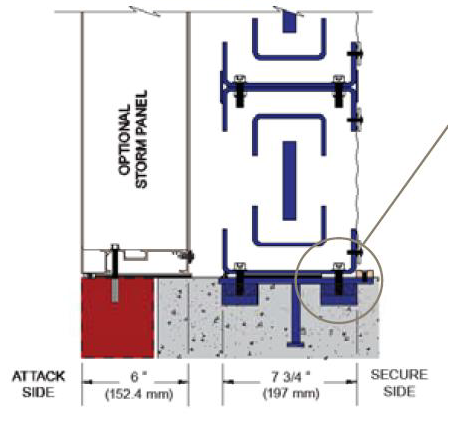
\includegraphics[width=.45\textwidth]{CrossSection}
			\caption{Cross-section of example FEBR louver}
			\label{fig:CSec}
		\end{figure}
		
		Air is allowed to flow between the right and left sides, however there is no pathway for ballistic projectiles to pass through and injure the occupants or damage equipment.  To the left of the FEBR louver is a storm shutter that is closed in inclement weather to prevent water entering the structure.
		
		The FEBR louver was designed and optimized for minimal mass under three different loading conditions:
		\begin{itemize}
			\item a 1000 psi (pounds per square inch) load on the exterior faces
			\item a non-linear load focused over a circular projection with a maximum of 1000 psi at the center of the louver
			\item a 9-mm handgun bullet impacting the external faces of the louver
		\end{itemize}
		
		The labels for the various sections of the FEBR louver are labelled in Figure \ref{fig:Labels}.  The sections are the center, Level 1, and Level 2.  The tabs associated with the different levels are visible going vertically. \nopagebreak[4] \begin{figure}[H]
			\centering
			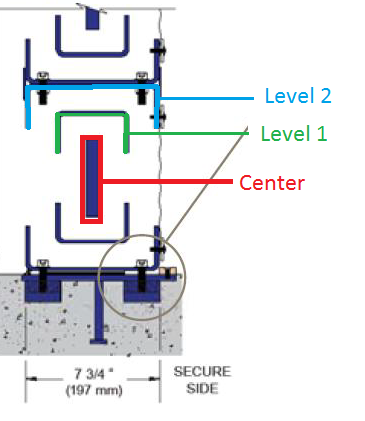
\includegraphics[width=.45\textwidth]{Labelled}
			\caption{Labelled FEBR louver}
			\label{fig:Labels}
		\end{figure}
		
		\newpage
		\section{Major Requirements}
		There are several main requirements for the louver:
		\begin{itemize}
			\item The total deflection in any loading condition can be no larger than $0.5\inchsign$
			\item There must be at least a 1-inch gap between all interior surfaces to allow for airflow
			\item The louver must be $7\sfrac{3}{4}\inchsign$ wide (in the direction of airflow)
			\item The louver must be $50\inchsign$ long.  Note that in many depictions of the louver, this will be coming out of the page
			\item The general shape of the louver must not be drastically altered from Figure \ref{fig:CSec}
			\item From the front view, there can be no open sections of the louver to prevent projectiles from passing through
			\item The wall thickness of any part can be no less than $\sfrac{1}{8}\inchsign$
			\item All design and analysis must be done in Pro/ENGINEER and Pro/Mechanica
		\end{itemize}
		
		
		\chapter{FEBR Louver}
		\vspace{-.25in}
		\section{Parametric Design}
		To simplify and expedite the optimization process, several simplifications were used.  First, and most visibly, fillets were not implemented in the models.  This reduced the number of elements in the meshing and finite element analyses by several thousand, from roughly 2,000 to roughly 600.  The fillets reduced the stresses by roughly a factor of 5\%, lower than the margin of error in the stress analyses performed in Pro/Mechanica of 10\%.
		
		An additional simplification that was performed was splitting the model of the louver into three separate ones that were each then individually optimized, instead of optimizing the parts together.  The significantly reduced number of elements greatly reduced the computation time.
		
		The optimizations were also performed on either half or a quarter of the final product.  The louver exhibits symmetry about a horizontal plane running through its middle and a vertical plane whose normal vector points along the left-right axis.  The planes of symmetry are visible in Figure \ref{fig:Symmetry}
		
		\begin{figure}[H]
			\centering
			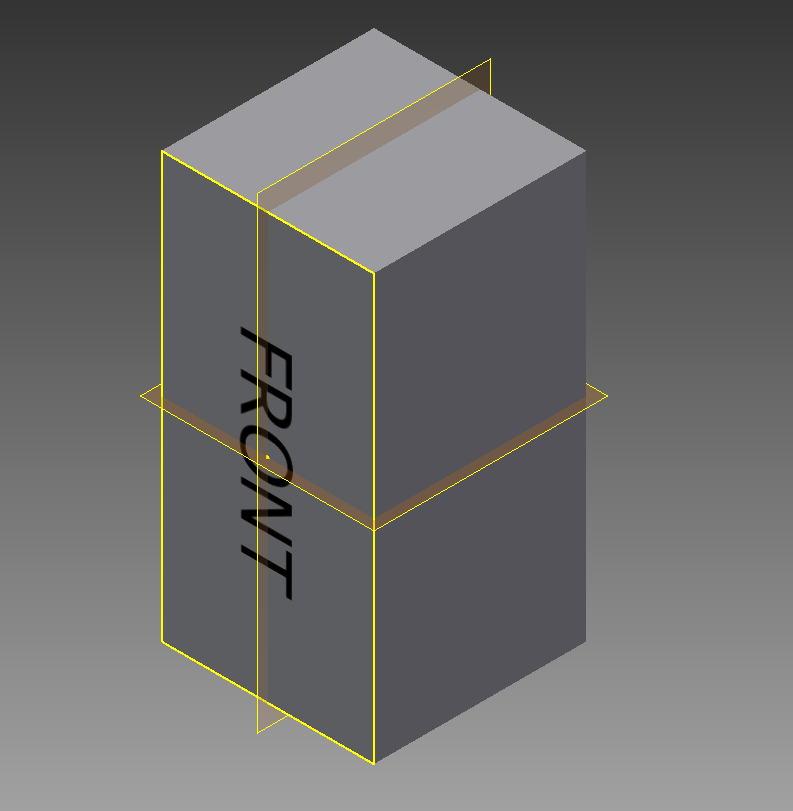
\includegraphics[width=.45\textwidth]{Symmetry}
			\caption{Visual representation of symmetric planes}
			\label{fig:Symmetry}
		\end{figure}
		
		This symmetry allows the center piece to be modelled with the top left corner and have two symmetry constrains applied in Pro/ENGINEER Mechanica.  The outer layers could be modelled with just the top half.  The center piece and its symmetry constrains can be seen in Figure \ref{fig:SymmetryConstrains}.  The symmetry constrains are the half-blue boxes on the right side and the bottom of the model.

		\graphicspath{ {./ScreenShots/Sinusoidal/} }
		\begin{figure}[h!]
			\centering
			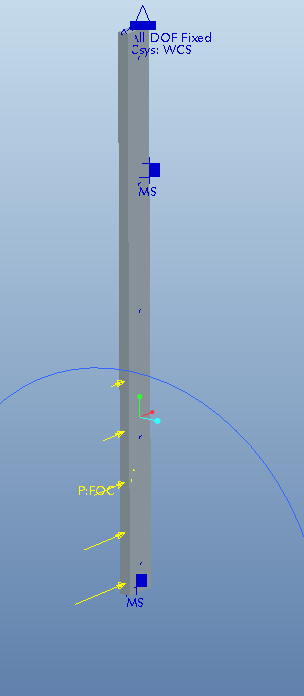
\includegraphics[width=.25\textwidth]{WaveForceCenterSetUp}
			\caption{Center section of FEBR louver and symmetry constraints}
			\label{fig:SymmetryConstrains}
		\end{figure}
		\graphicspath{ {..} }
		
		To simulate being installed in their final location, the top and bottom of the FEBR louver are fixed, allowing neither rotation nor translation.  This approximates the louvers being welded in their location.  If the joints were pinned, then the beams would have had to be significantly thicker.
		
		\subsection{Center}
		The thickness of the center piece was not varied but rather it was kept at $1.0\inchsign$.  The minimum separation between any two surfaces of the louver is $1.0\inchsign$.  Since the edges of the next layer cannot be closer than $1.0\inchsign$ and a bullet cannot be able to go straight through, the minimum thickness of the center beam is $1.0\inchsign$.  An increase in the frontal area of the beam would increase the deflection, as opposed to minimizing it.  The additional material in the beam does not offset the increased forces from the pressure loads.  Furthermore, keeping the beam long and narrow increased its second moment of area, given in Equation \ref{eq:SecondMomentofArea}.
		
		\begin{equation}
		I_y = \int\limits_{A} x^2 \: \mathrm{d}A = \frac{h b^3}{12}
		\label{eq:SecondMomentofArea}
		\end{equation}
		
		Here, $b$ is the length of the beam (variable) and $h$ is the thickness (held constant).  Maximizing $b$ increases the beam's second moment of area, decreasing the deflection from bending, given below in Equation \ref{eq:Deflection}.
		
		\begin{equation}
		\delta = \frac{F L^3}{3 E I_y}
		\label{eq:Deflection}
		\end{equation}
		
		As you can see, increasing $I_y$ decreases $\delta$, the deflection.
		
		The beam could be no thinner than $0.125\inchsign$ and the maximum was $2\sfrac{1}{2}\inchsign$.  The maximum was determined through trial and error.  Roughly, when thicker than $2.0\sfrac{1}{2}\inchsign$, Level 2 could not be sufficiently thick to prevent its deflection when under severe loading.  The center was not limited by this maximum, however.  When optimized, the mass of the beam was minimized while maintaining less than $0.5\inchsign$ of deflection.
		
		\subsection{Level 1}
		The next closest part to the center is referred to as the first level, or Level 1.  Here, the bent over tabs are constrained to the center piece.  Since the center piece is defined to be an inch thick, the tabs are going to be an inch apart, adhering to the constraints given.  Figure \ref{fig:L1Constraints} highlights the collinear constraints for the tabs.
		
		\graphicspath{ {./ScreenShots/} }
		\begin{figure}[h]
			\centering
			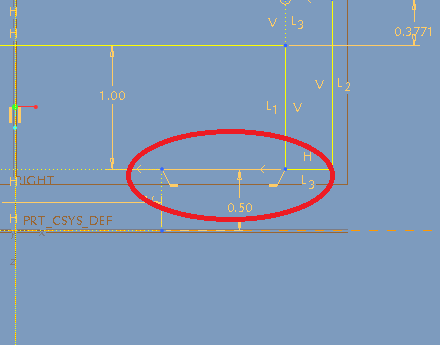
\includegraphics[width=.75\textwidth]{L1Constraints}
			\caption{Constraints for Level 1 tabs, highlighting the collinear one}
			\label{fig:L1Constraints}
		\end{figure}
		\graphicspath{ {..} }
		
		For Level 1, the thickness was varied from $\sfrac{1}{8}\inchsign$ to an arbitrarily high value.  This allowed the optimal value to be found without the limits interfering with the optimization's searching.
		
		The gaps between the center and Level 1 were also allowed to vary; $1.0\inchsign$ was the minimum and $2.0\inchsign$, an arbitrarily large value, was the maximum.
		
		\subsection{Level 2}
		The outermost layer, Level 2, surrounds both Level 1 and the center piece.  It is required that Level 2 be $7\sfrac{3}{4}\inchsign$ wide.  Again, the tabs were collinearly constrained to the top side of Level 1.  The spacing between the outer edge of Level 1 and the inner edge of Level 2 was varied from the air-flow minimum of $1.0\inchsign$ to a maximum such that the thickness of Level 2 was not less than the minimum of $\sfrac{1}{8}\inchsign$.
		
		The length of the exterior tabs were also allowed to vary from $1.0\inchsign$ to an arbitrarily large value of $3.0\inchsign$.  The separation between Level 2 and Level 1 was limited to exactly $1.0\inchsign$.
		
		\section{Finite Element Model}
		Meshes for Finite Element Analysis (FEA) were created in Mechanica using AutoGEM.  Since the models that were being analyzed are all rectangular or made up of rectangular blocks, the meshes were very simple.  Furthermore, the default settings for AutoGEM produced acceptable meshes for the center, Level 1, and Level 2.
		
		Figure \ref{fig:CenterMesh} shows the mesh for the center section with 44 elements.  Figure \ref{fig:L1Mesh} shows the mesh for the Level 1 section with 131 elements.  Figure \ref{fig:L2Mesh} shows the mesh for the Level 2 section with 110 elements.
		
		\graphicspath{ {./ScreenShots/Meshes/} }
		\begin{figure}[H]
			\centering
			\begin{subfigure}{.3\textwidth}
				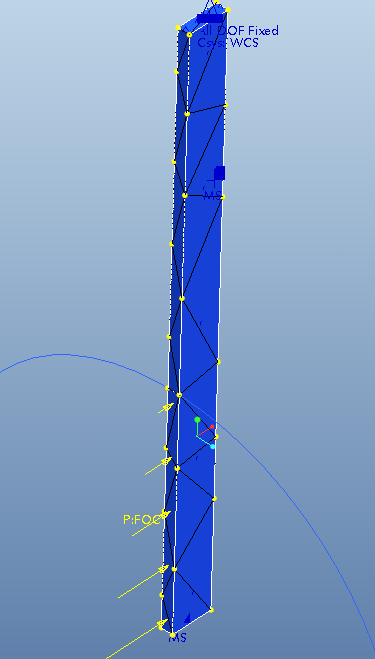
\includegraphics[width=\textwidth]{CenterMeshCrop}
				\subcaption{Mesh of center section}
				\label{fig:CenterMesh}
			\end{subfigure}
			\begin{subfigure}{.3\textwidth}
				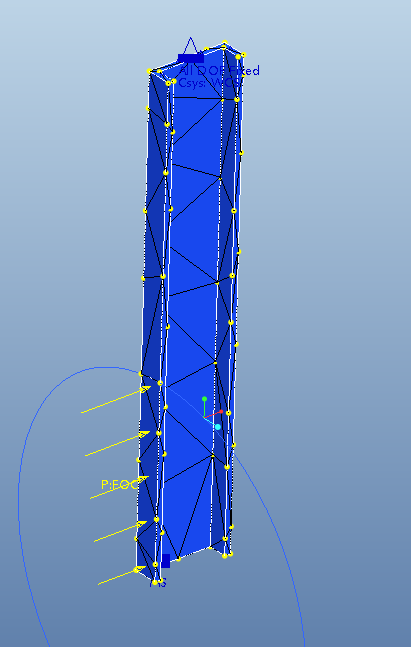
\includegraphics[width=\textwidth]{L1MeshCrop}
				\subcaption{Mesh of Level 1}
				\label{fig:L1Mesh}
			\end{subfigure}
			\begin{subfigure}{.3\textwidth}
				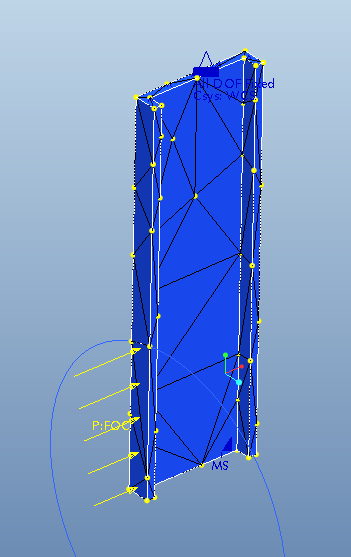
\includegraphics[width=\textwidth]{L2MeshCrop}
				\subcaption{Mesh of Level 2}
				\label{fig:L2Mesh}
			\end{subfigure}
			\caption{Finite element meshes}
		\end{figure}
		\graphicspath{ {..} }
		
		Table \ref{tab:SummarOfElements} presents a summary of the items and their number of elements.
		
		\begin{table}[H]
			\centering
			\begin{tabular}{|c|c|}
			\hline \textbf{Item} & \textbf{Number of Elements}\\
			\hline Center & 44\\
			\hline Level 1 & 131\\
			\hline Level 2 & 110\\
			\hline
			\end{tabular}
			\caption{Summary of elements in finite element model}
			\label{tab:SummarOfElements}
		\end{table}
		
		\subsection{Element Types, Loads, and Boundary Conditions}
		For the bullet, the load was a 90-kN load spread over a circle with a 9mm diameter.  The reasoning behind the determination of this load is discussed later.  For the center, since the bullet is impacting its middle, instead of a circle, the load is applied over a quarter-circle.  Since the simplified area is a quarter of the full, the load applied is $22\sfrac{1}{2}$ kN.
		
		For the pressure, a simple pressure load of 1000 psi (or 1 ksi) was applied along the five exterior faces.
		
		For the more advanced pressure load, it was applied in a 20-inch diameter circle.  At the center, the load was 1000 psi and along the circumference of the circle, the load was zero.  The load followed Equation \ref{eq:force}.
		
		\begin{align}
		F = 500\left[\cos\left(\frac{\pi r}{10}\right) +1 \right]
		\label{eq:force}
		\intertext{Where:}
		r = \sqrt{y^2+z^2}
		\end{align}
		
		Note that the force is a function of $y$ and $z$.  Since the force is distributed over a circular area, at the limits of the circle, the load is equal to zero pounds.  Figure \ref{fig:forceplot} shows a 3-dimensional plot of the force generated in MATLAB for the force described in Equation \ref{eq:force}.  Note that the z-axis is the force in pounds per square inch (psi).
		
		\begin{figure}[H]
			\centering
			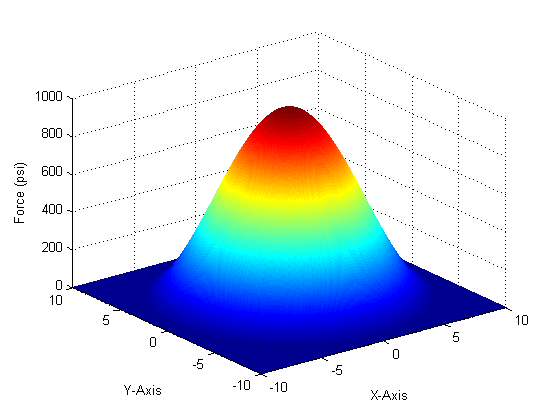
\includegraphics[width=.75\textwidth]{ForcePlot}
			\caption{Plot of the sinusoidal force}
			\label{fig:forceplot}
		\end{figure}
		
		For the MATLAB code used to plot this, see Appendix A.
		
		\subsection{Analysis of 9-mm Handgun Bullet}
		
		Assuming that the bullet is a standard 9x19mm Parabellum bullet, the fastest the 7.45 gram projectile can go is 435 $\sfrac{m}{sec}$.\footcite{wiki:9mm}  This gives it 704 Joules of energy at impact, assuming no frictional losses during flight.  The force imparted is approximated by combining the concepts of conservation of momentum and impulses.
		
		There are several assumptions that were made to get a rough approximation of the behavior of a bullet.
		\begin{itemize}
			\item The bullet is fired under point-blank firing conditions, giving a worst-case scenario for damage to the louver
			\item The bullet is brought completely to rest during its impact with the louver
			\item The bullet stops over its total length
		\end{itemize}
		
		All of the bullet's forward momentum must be cancelled out by an impulse given from the wall.  This gives us the following equation:
		
		\begin{equation}
		m \Delta v = F \Delta t
		\label{eq:momentum-impulse}
		\end{equation}
		
		where $m$ is the mass of the bullet, $\Delta v$ is the change of the bullet's velocity, $F$ is the force imparted on the bullet by the wall, and $\Delta t$ is the time over which the force is imparted.
		
		Since the bullet stops completely over its length, the time taken can be roughly approximated by calculating the time that it takes for the bullet to travel its own length.  This is given by the equation:
		
		\begin{equation}
		\Delta t = \frac{l}{v}
		\end{equation}
		
		where $l$ is the length of the bullet and $v$ is its velocity.  The length of a 9mm bullet is 15.7 mm, giving the stopping time to be 3.6\e{-5} seconds (\mbox{36 $\mu s$}).\footcite{pic:9mm}
		
		Rearranging Equation \ref{eq:momentum-impulse} with the numbers now known, we can determine the force experienced by the bullet from the louver:
		
		\begin{align*}
		F &= \frac{m \Delta v}{\Delta t}\\
		&=\frac{(7.45\e{-3}\textrm{ kg})(435 \textrm{ } \sfrac{m}{sec})}{3.6\e{-5} \textrm{ sec}}\\
		&\approx 9\e{4} \textrm{ N}\\
		&= 90 \textrm{ kN}
		\end{align*}
		
		This 90 kN number was used in the calculations for the bullet impact's effects.
		
		\newpage
		\section{Convergence}
		The center, Level 1, and Level 2 were optimized separately.  Each optimization that was run could be completed quickly and the results verified.  Multiple optimizations were run.  As an example, several graphs were generated from the part's displacement and total mass.  These two parameters were chosen because the displacement has a maximum and we are attempting to minimize the mass; we are interested in both parameters.  While it may be difficult to see in these thumbnail images, the displacement during the final iteration is around $0.5\inchsign$, within Pro/ENGINEER's margin of error.
		
		\begin{center}
			\vfill
			\begin{scriptsize}
				This space intentionally left blank
			\end{scriptsize}
		\end{center}
		
		\newpage
		\subsection{Bullet Load}
		\graphicspath{ {./ScreenShots/Bullet/} }
		\begin{figure}[H]
			\centering
			\begin{subfigure}{.45\textwidth}
				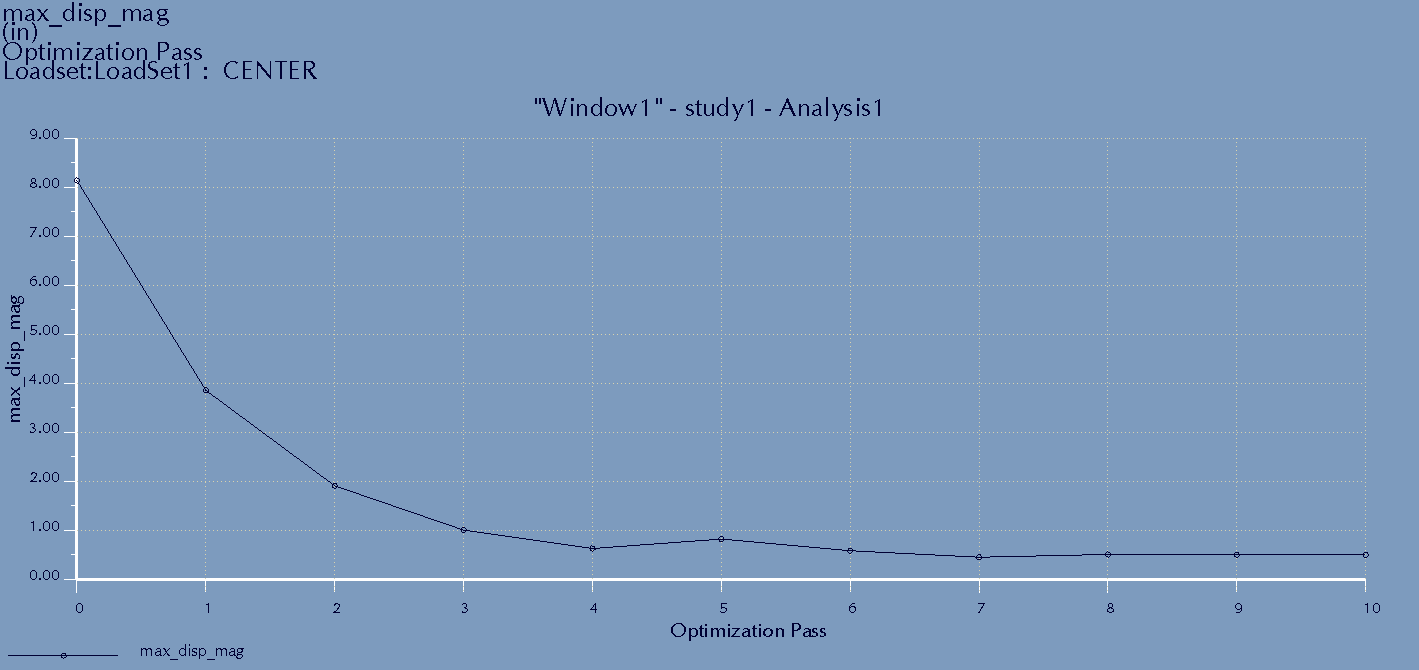
\includegraphics[width=\textwidth]{CenterBulletOptimDispGraph}
				\subcaption{Displacement}
				\label{fig:CenterBulletOptimDispGraph}
			\end{subfigure}
			\begin{subfigure}{.45\textwidth}
				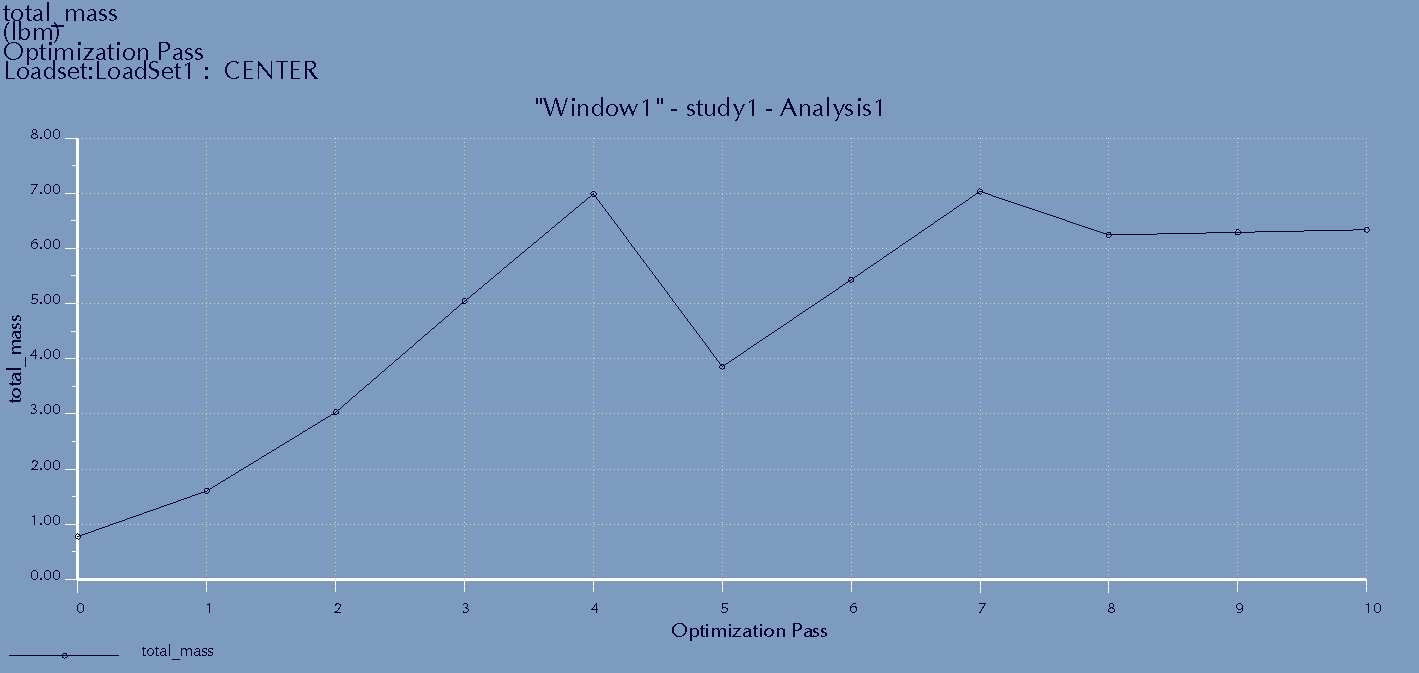
\includegraphics[width=\textwidth]{CenterBulletOptimMassGraph}
				\subcaption{Mass}
				\label{fig:CenterBulletOptimMassGraph}
			\end{subfigure}
			\caption{Optimization of center under bullet load}
		\end{figure}
		
		\begin{figure}[H]
			\centering
			\begin{subfigure}{.45\textwidth}
				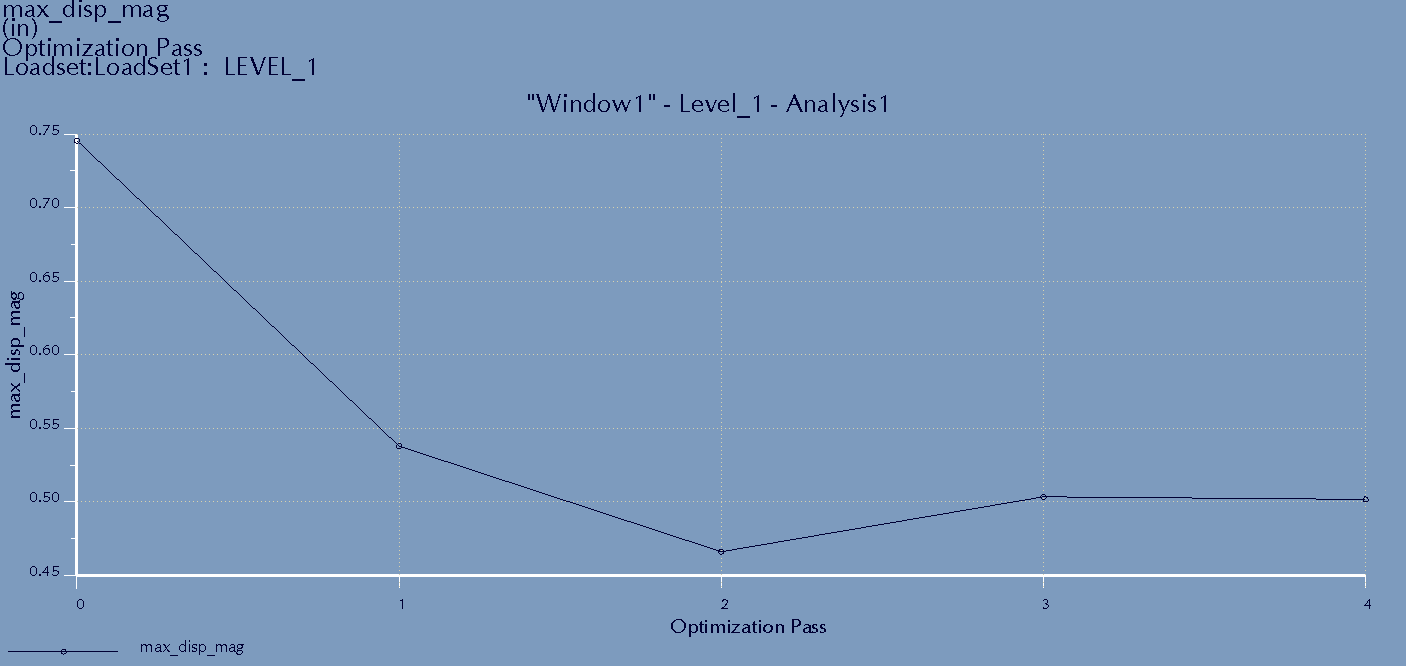
\includegraphics[width=\textwidth]{L1BulletOptimDispGraph}
				\subcaption{Displacement}
				\label{fig:L1BulletOptimDispGraph}
			\end{subfigure}
			\begin{subfigure}{.45\textwidth}
				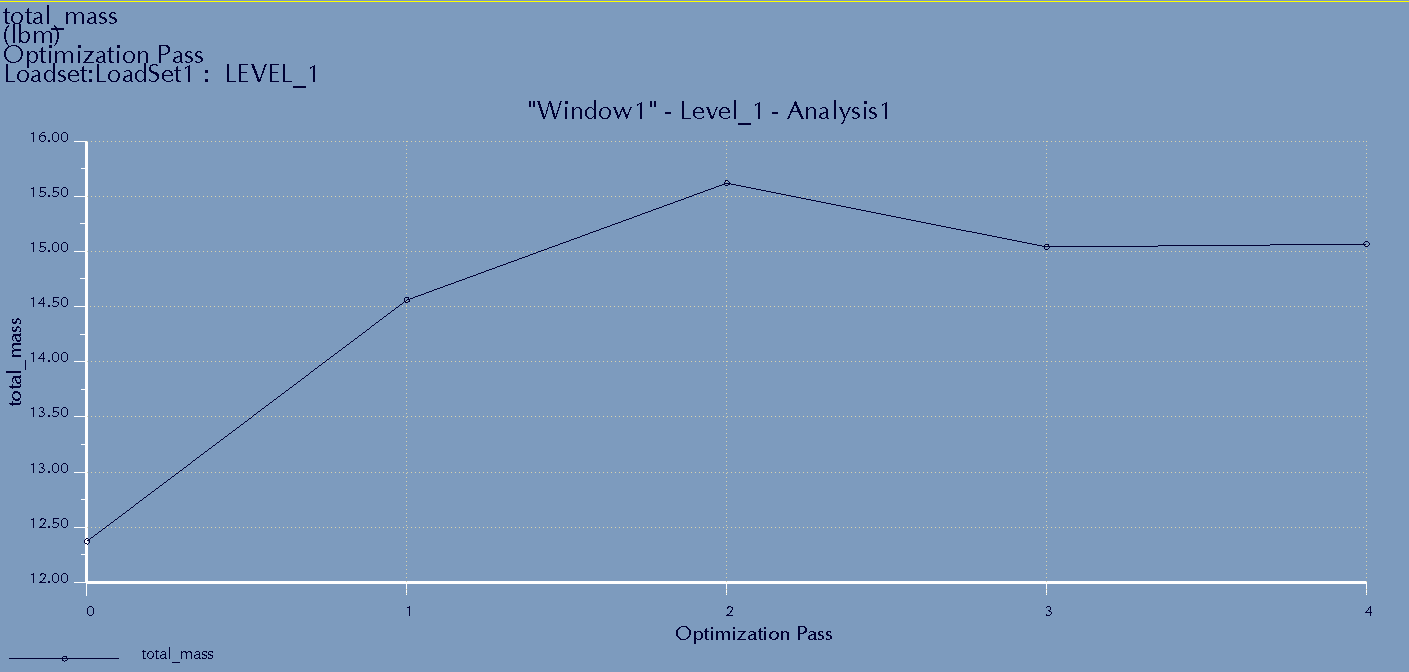
\includegraphics[width=\textwidth]{L1BulletOptimMassGraph}
				\subcaption{Mass}
				\label{fig:L1BulletOptimMassGraph}
			\end{subfigure}
			\caption{Optimization of Level 1 under bullet load}
		\end{figure}
		
		\begin{figure}[H]
			\centering
			\begin{subfigure}{.45\textwidth}
				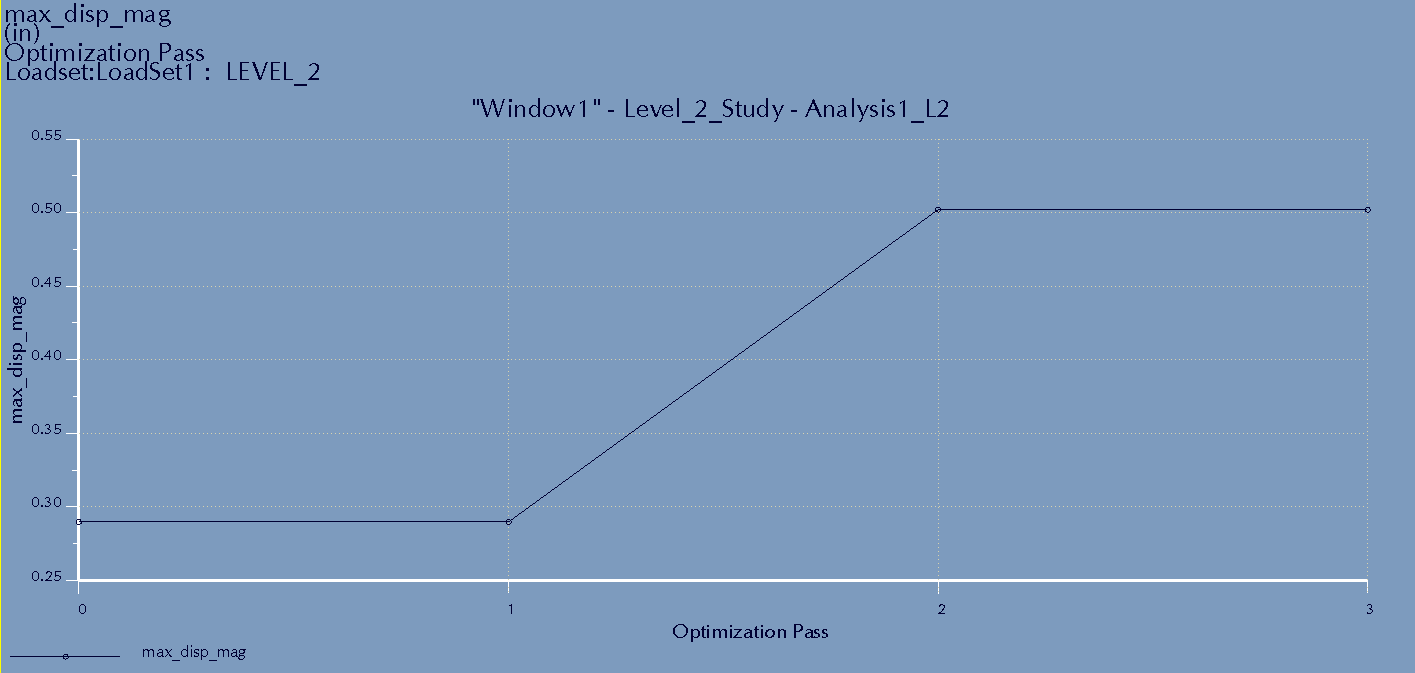
\includegraphics[width=\textwidth]{L2BulletOptimDispGraph}
				\subcaption{Displacement}
				\label{fig:L2BulletOptimDispGraph}
			\end{subfigure}
			\begin{subfigure}{.45\textwidth}
				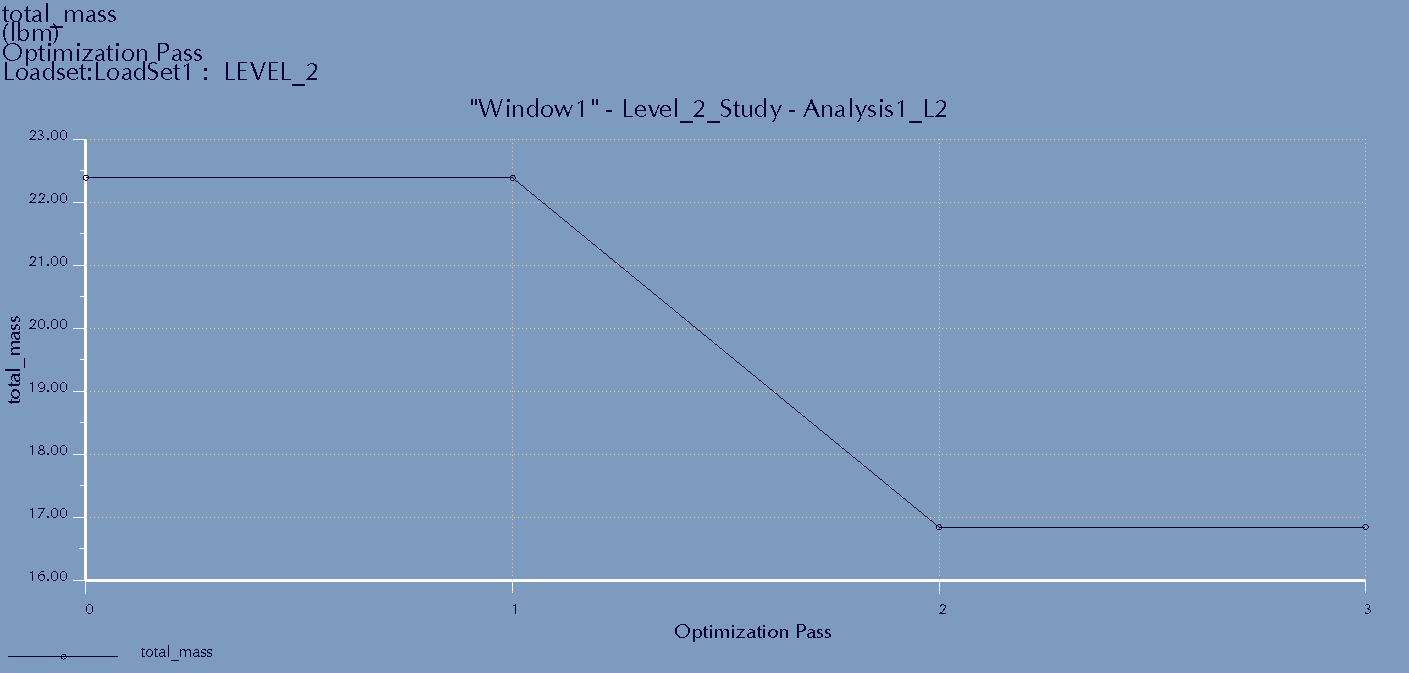
\includegraphics[width=\textwidth]{L2BulletOptimMassGraph}
				\subcaption{Mass}
				\label{fig:L2BulletOptimMassGraph}
			\end{subfigure}
			\caption{Optimization of Level 2 under bullet load}
		\end{figure}
		\graphicspath{ {..} }
		
		\newpage
		\subsection{Constant Pressure Load}
		\graphicspath{ {./ScreenShots/Pressure/} }
		\begin{figure}[H]
			\centering
			\begin{subfigure}{.45\textwidth}
				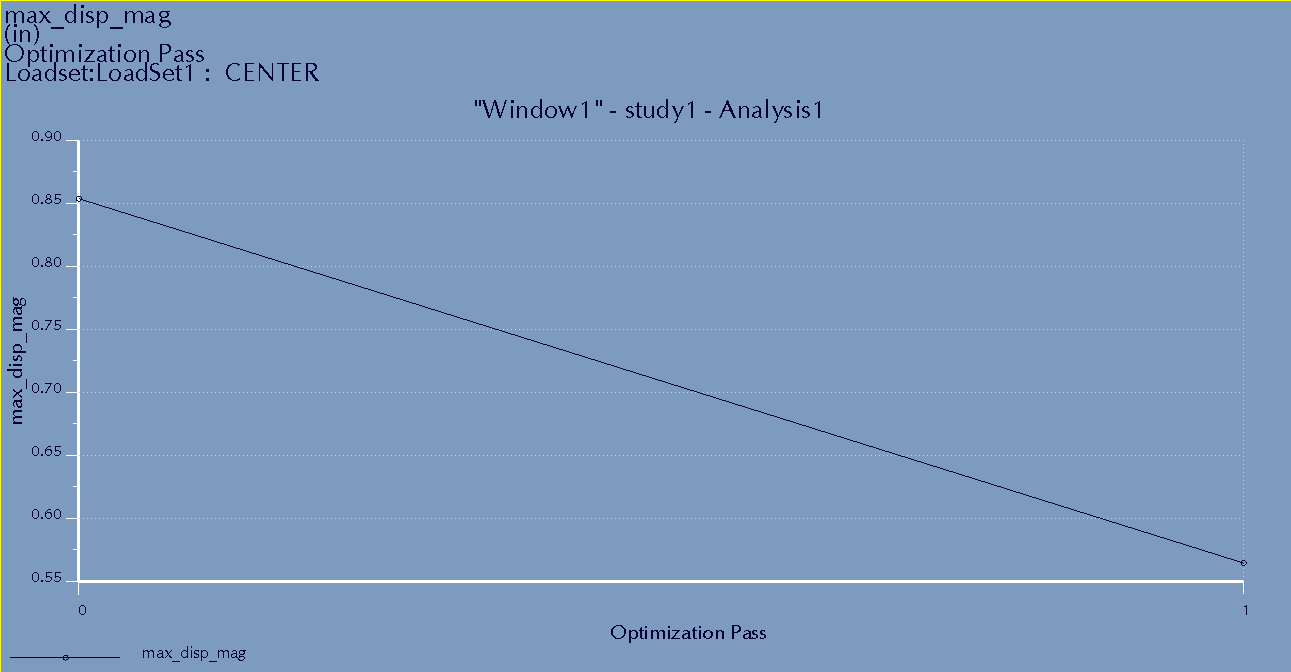
\includegraphics[width=\textwidth]{CenterOptimDisp}
				\subcaption{Displacement}
				\label{fig:CenterPressureOptimDispGraph}
			\end{subfigure}
			\begin{subfigure}{.45\textwidth}
				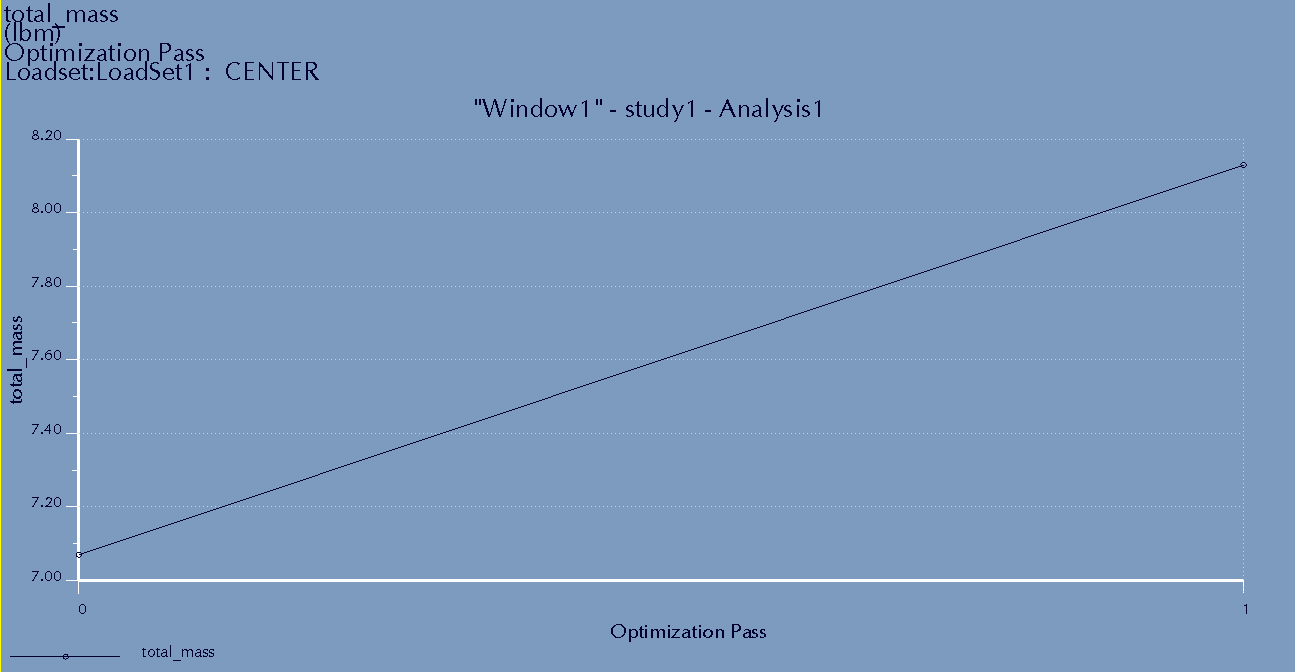
\includegraphics[width=\textwidth]{CenterOptimMass}
				\subcaption{Mass}
				\label{fig:CenterPressureOptimMassGraph}
			\end{subfigure}
			\caption{Optimization of center under constant pressure load}
		\end{figure}
		
		\begin{figure}[H]
			\centering
			\begin{subfigure}{.45\textwidth}
				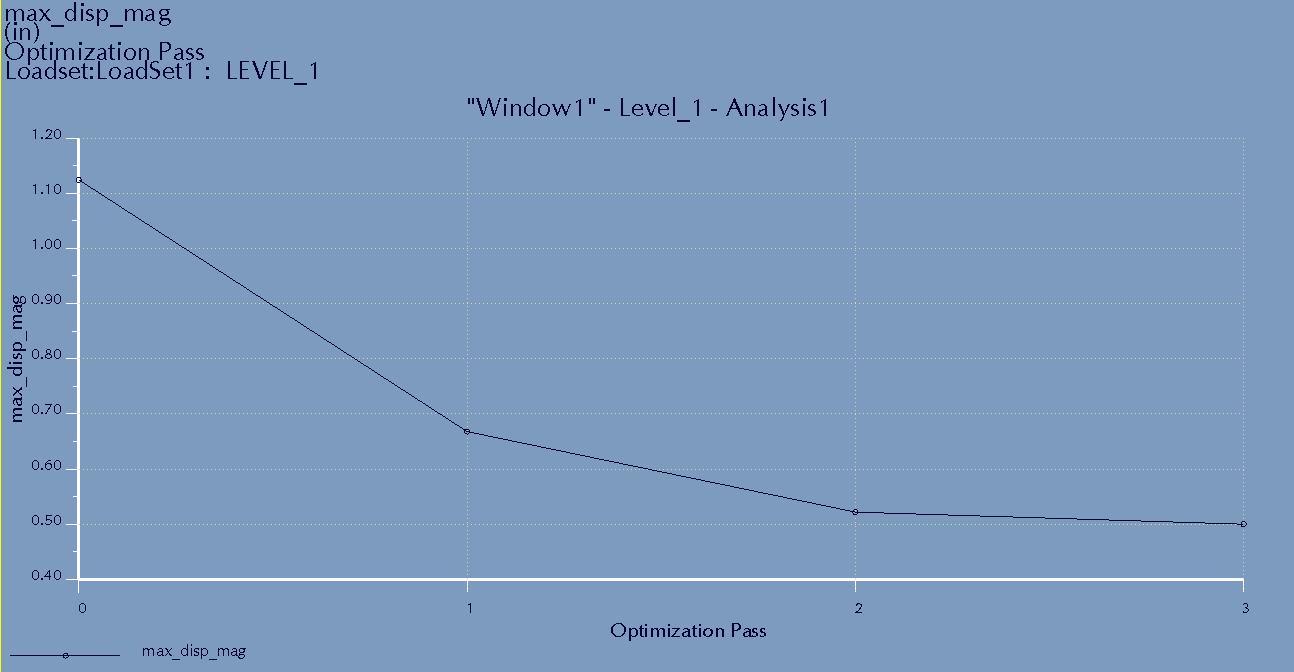
\includegraphics[width=\textwidth]{L1OptimDisp}
				\subcaption{Displacement}
				\label{fig:L1PressureOptimDispGraph}
			\end{subfigure}
			\begin{subfigure}{.45\textwidth}
				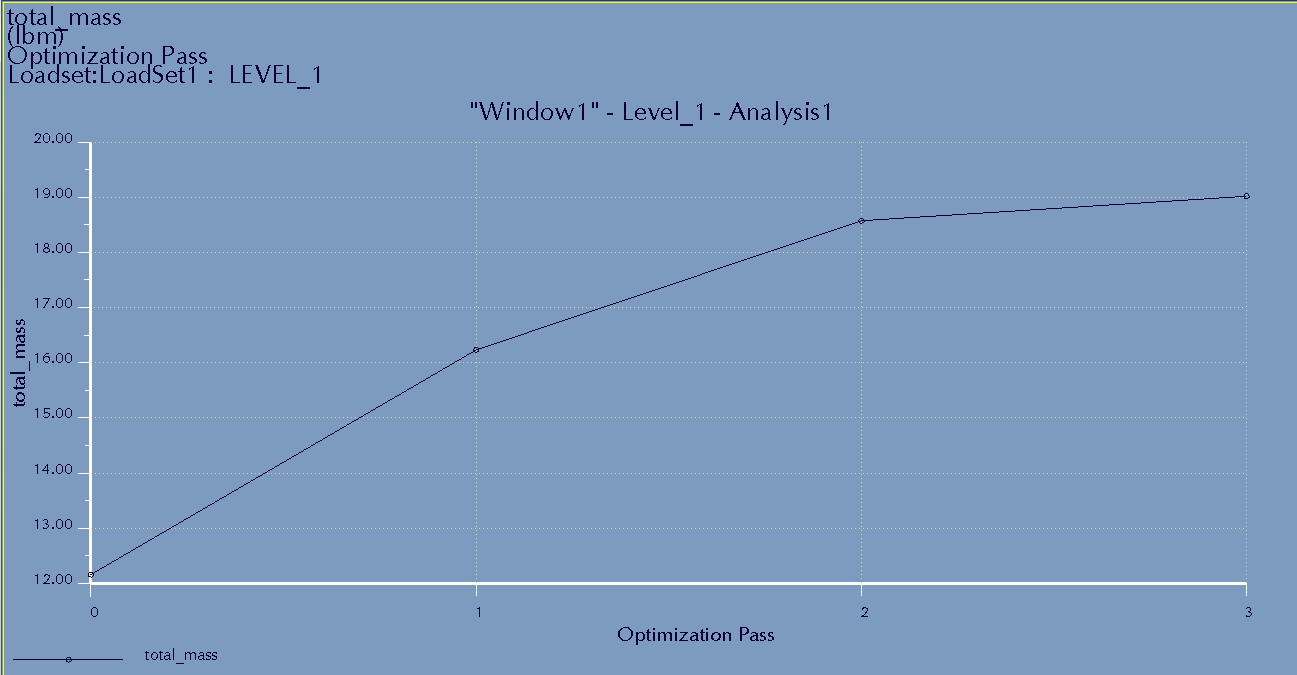
\includegraphics[width=\textwidth]{L1OptimMass}
				\subcaption{Mass}
				\label{fig:L1PressureOptimMassGraph}
			\end{subfigure}
			\caption{Optimization of Level 1 under constant pressure load}
		\end{figure}
		
		\begin{figure}[H]
			\centering
			\begin{subfigure}{.45\textwidth}
				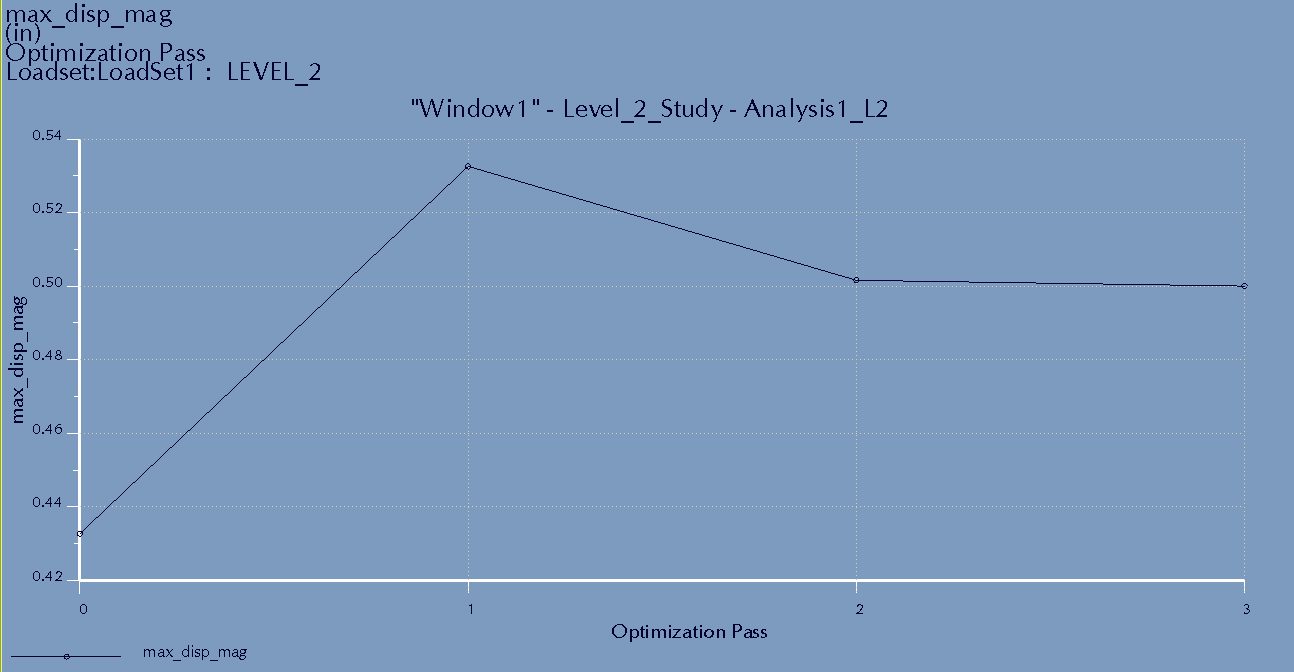
\includegraphics[width=\textwidth]{L2OptimDisp}
				\subcaption{Displacement}
				\label{fig:L2PressureOptimDispGraph}
			\end{subfigure}
			\begin{subfigure}{.45\textwidth}
				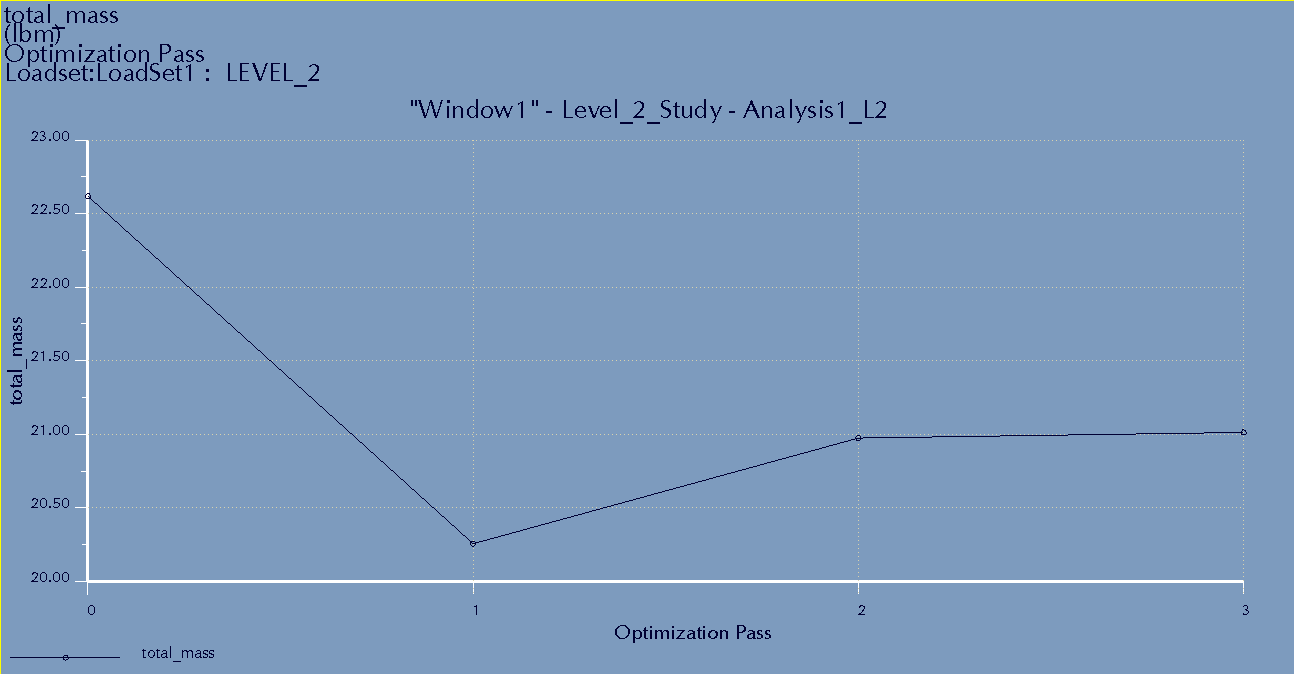
\includegraphics[width=\textwidth]{L2OptimMass}
				\subcaption{Mass}
				\label{fig:L2PressureOptimMassGraph}
			\end{subfigure}
			\caption{Optimization of Level 2 under constant pressure load}
		\end{figure}
		\graphicspath{ {..} }
		
		
		\newpage
		\subsection{Sinusoidal Pressure Load}
		\graphicspath{ {./ScreenShots/Sinusoidal/} }
		\begin{figure}[H]
			\centering
			\begin{subfigure}{.45\textwidth}
				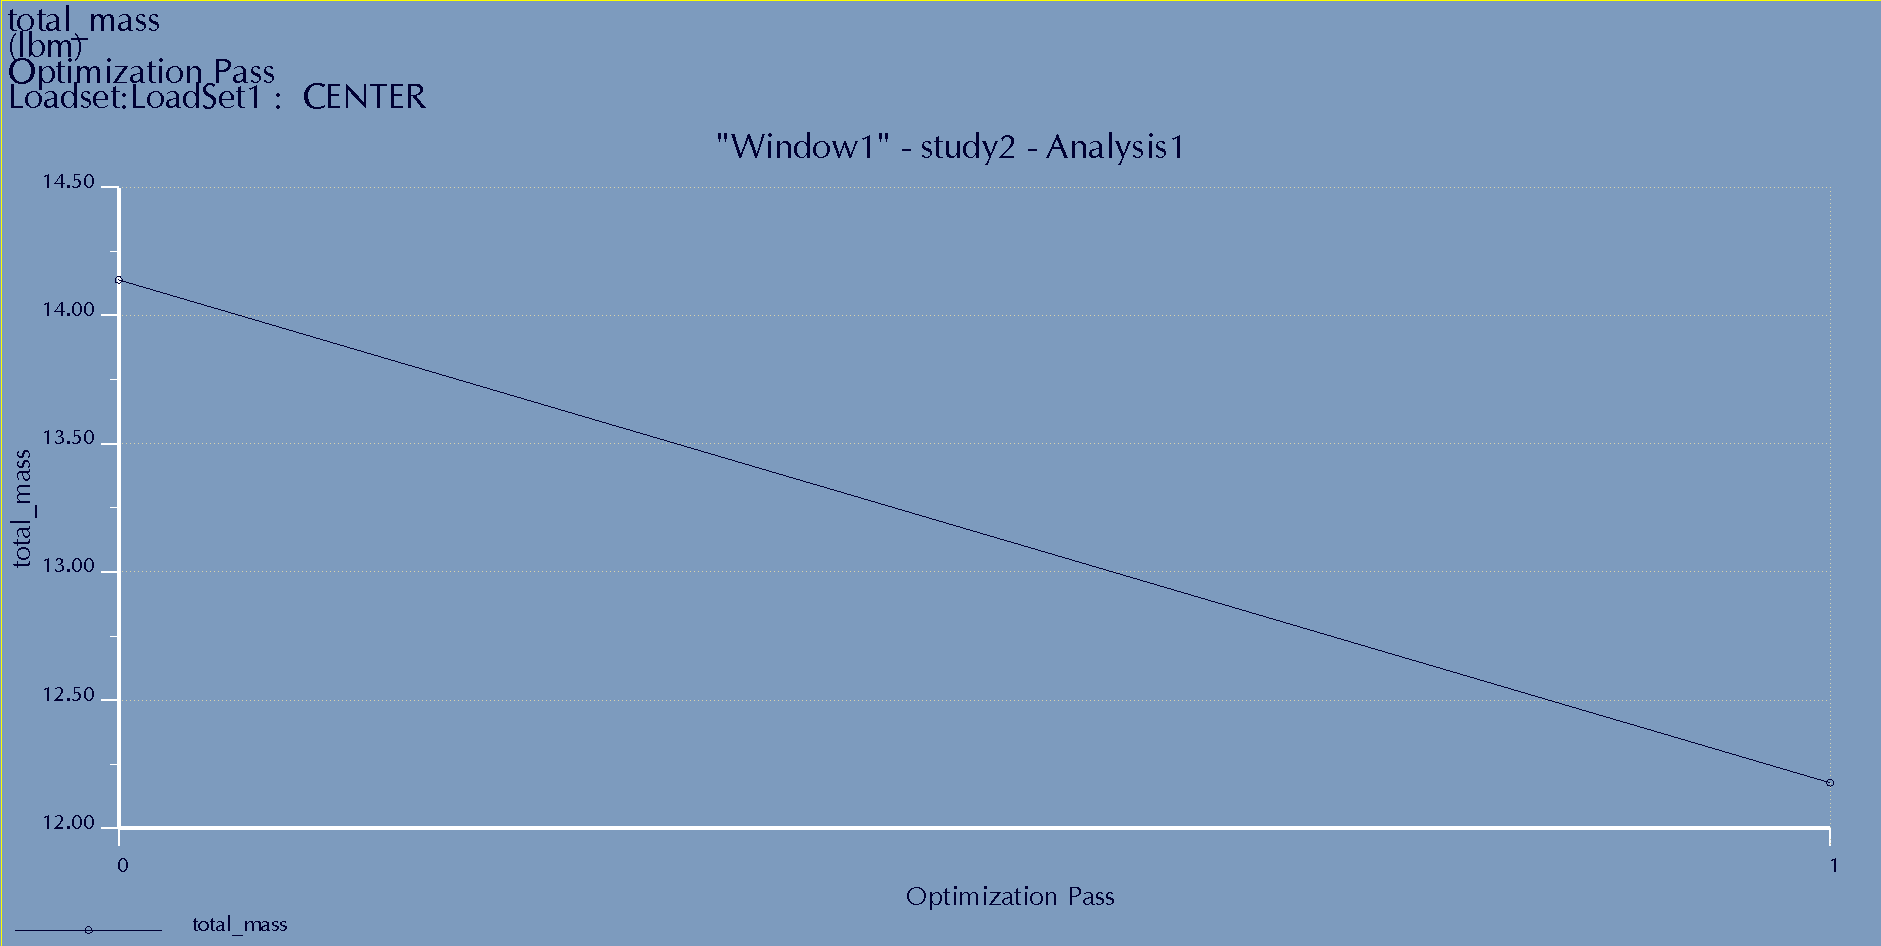
\includegraphics[width=\textwidth]{SinusoidalCenterOptimDisp}
				\subcaption{Displacement}
				\label{fig:CenterSinusoidalOptimDispGraph}
			\end{subfigure}
			\begin{subfigure}{.45\textwidth}
				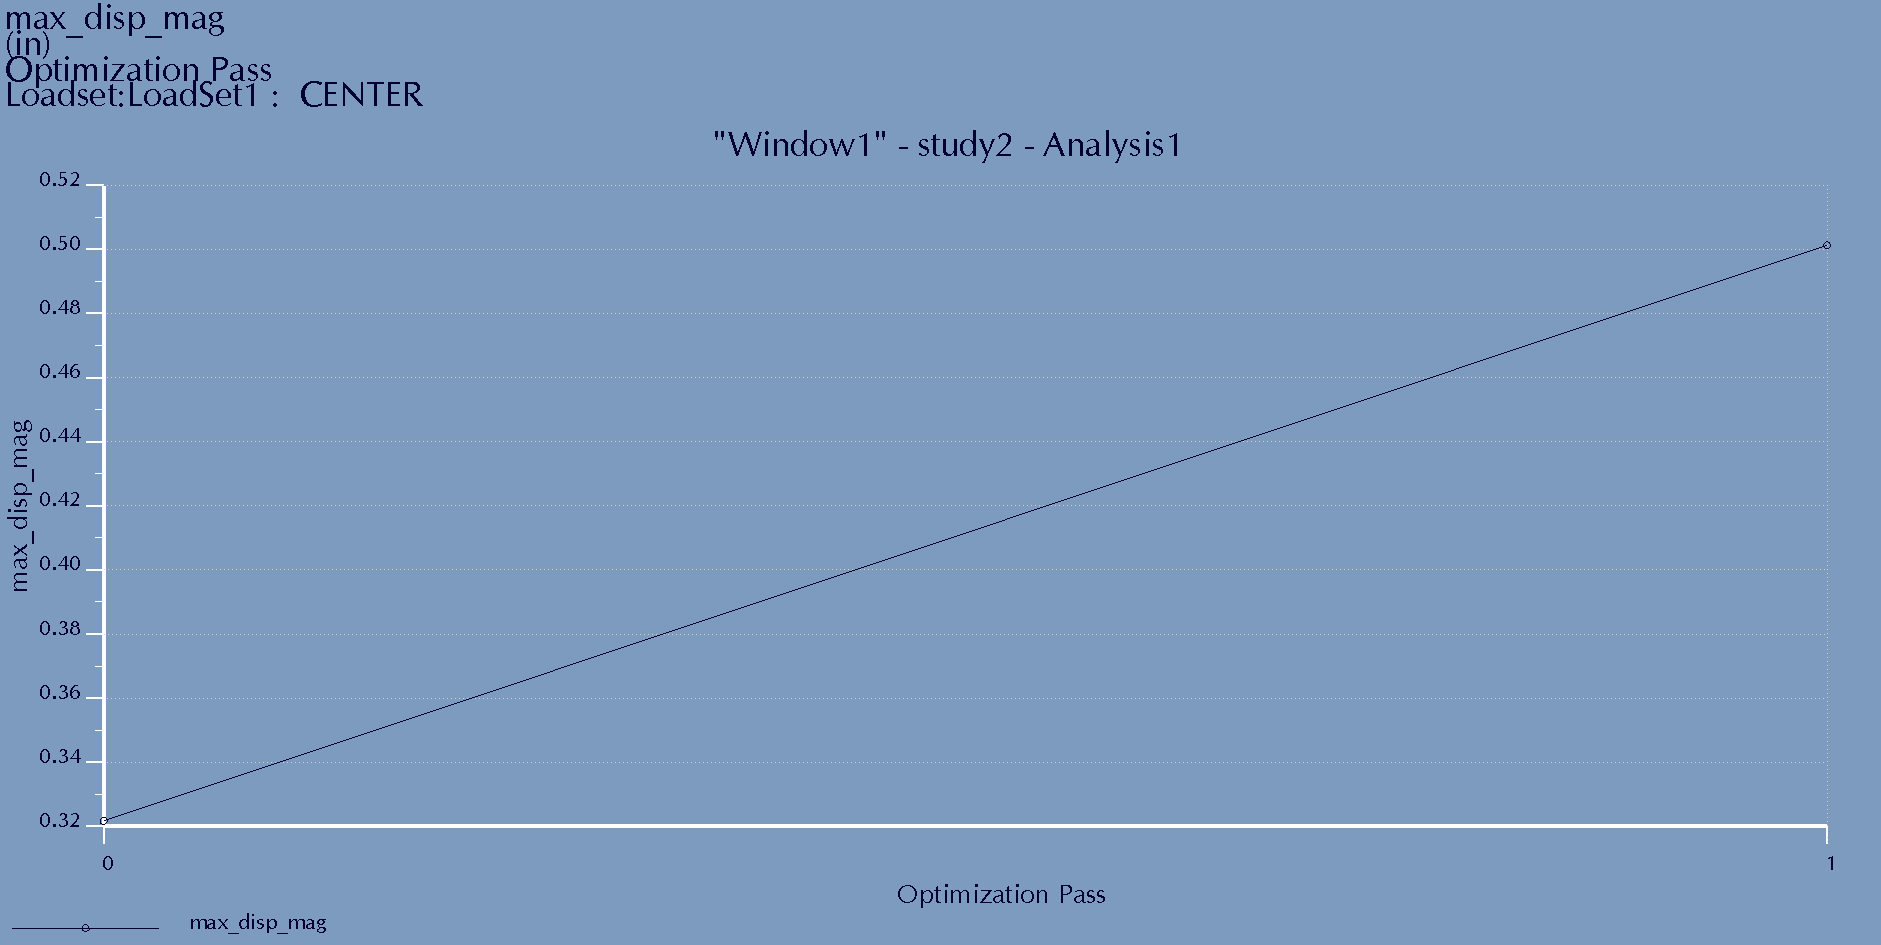
\includegraphics[width=\textwidth]{SinusoidalCenterOptimMass}
				\subcaption{Mass}
				\label{fig:CenterSinusoidalOptimMassGraph}
			\end{subfigure}
			\caption{Optimization of center under sinusoidal pressure load}
		\end{figure}
		
		\begin{figure}[H]
			\centering
			\begin{subfigure}{.45\textwidth}
				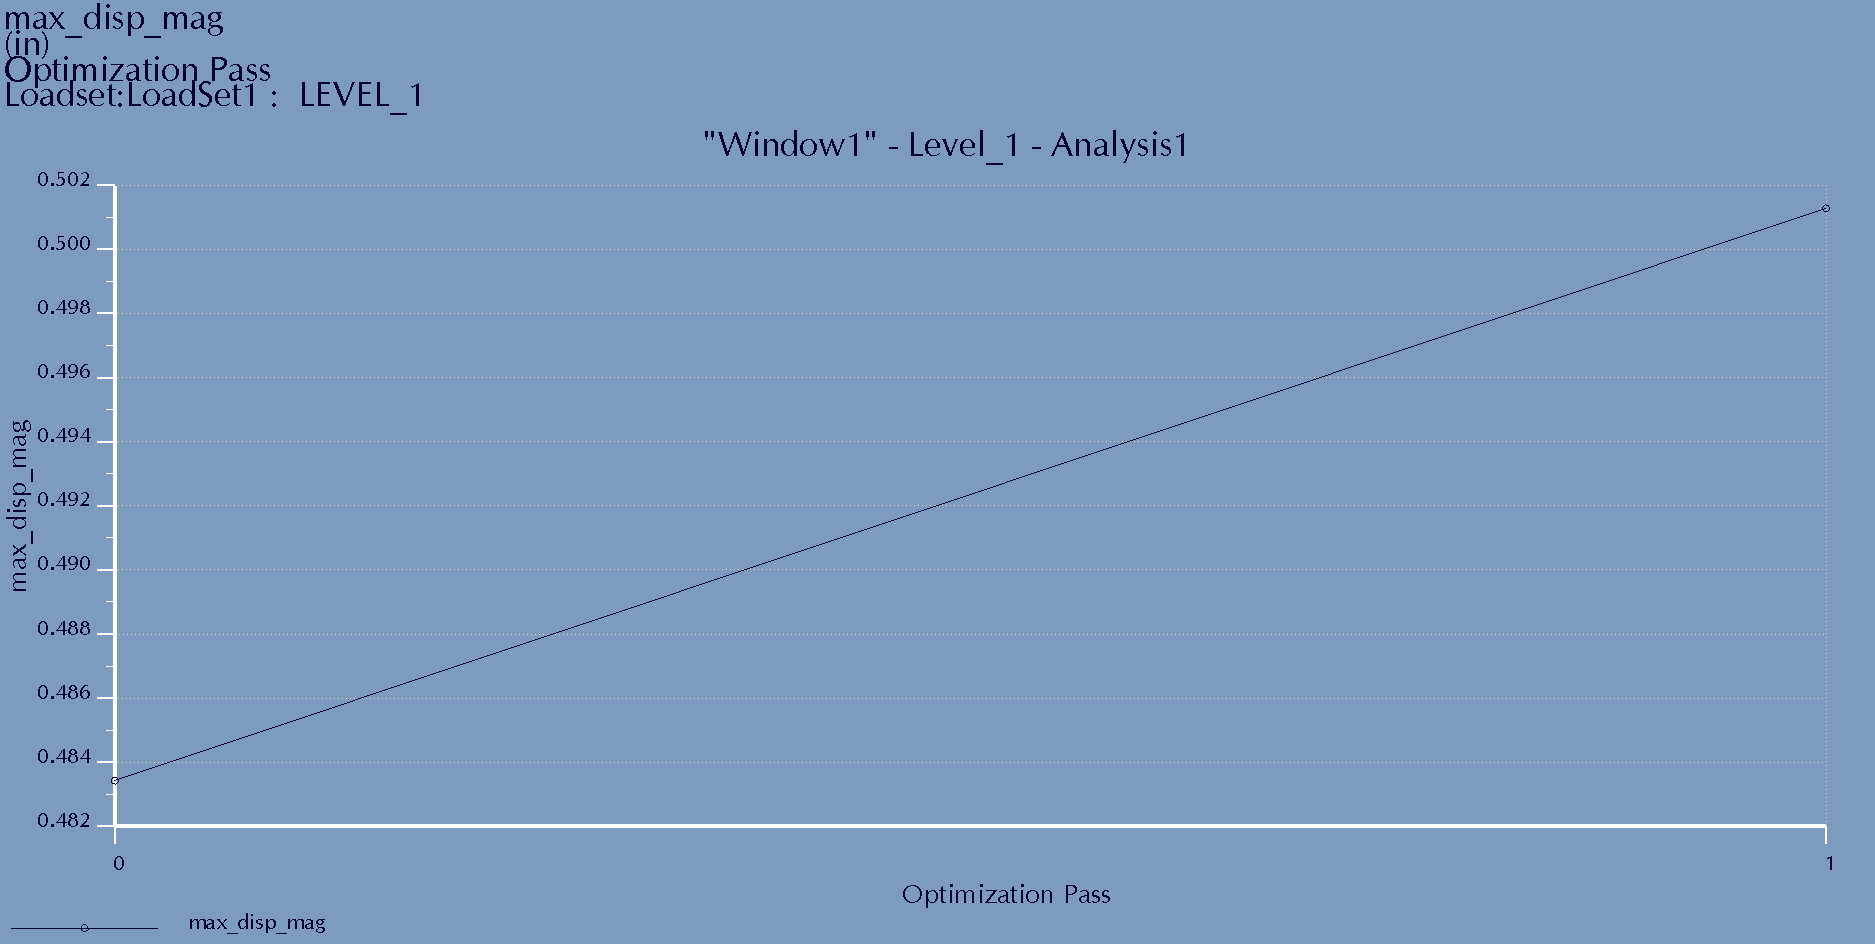
\includegraphics[width=\textwidth]{SinusoidalL1OptimDisp}
				\subcaption{Displacement}
				\label{fig:L1SinusoidalOptimDispGraph}
			\end{subfigure}
			\begin{subfigure}{.45\textwidth}
				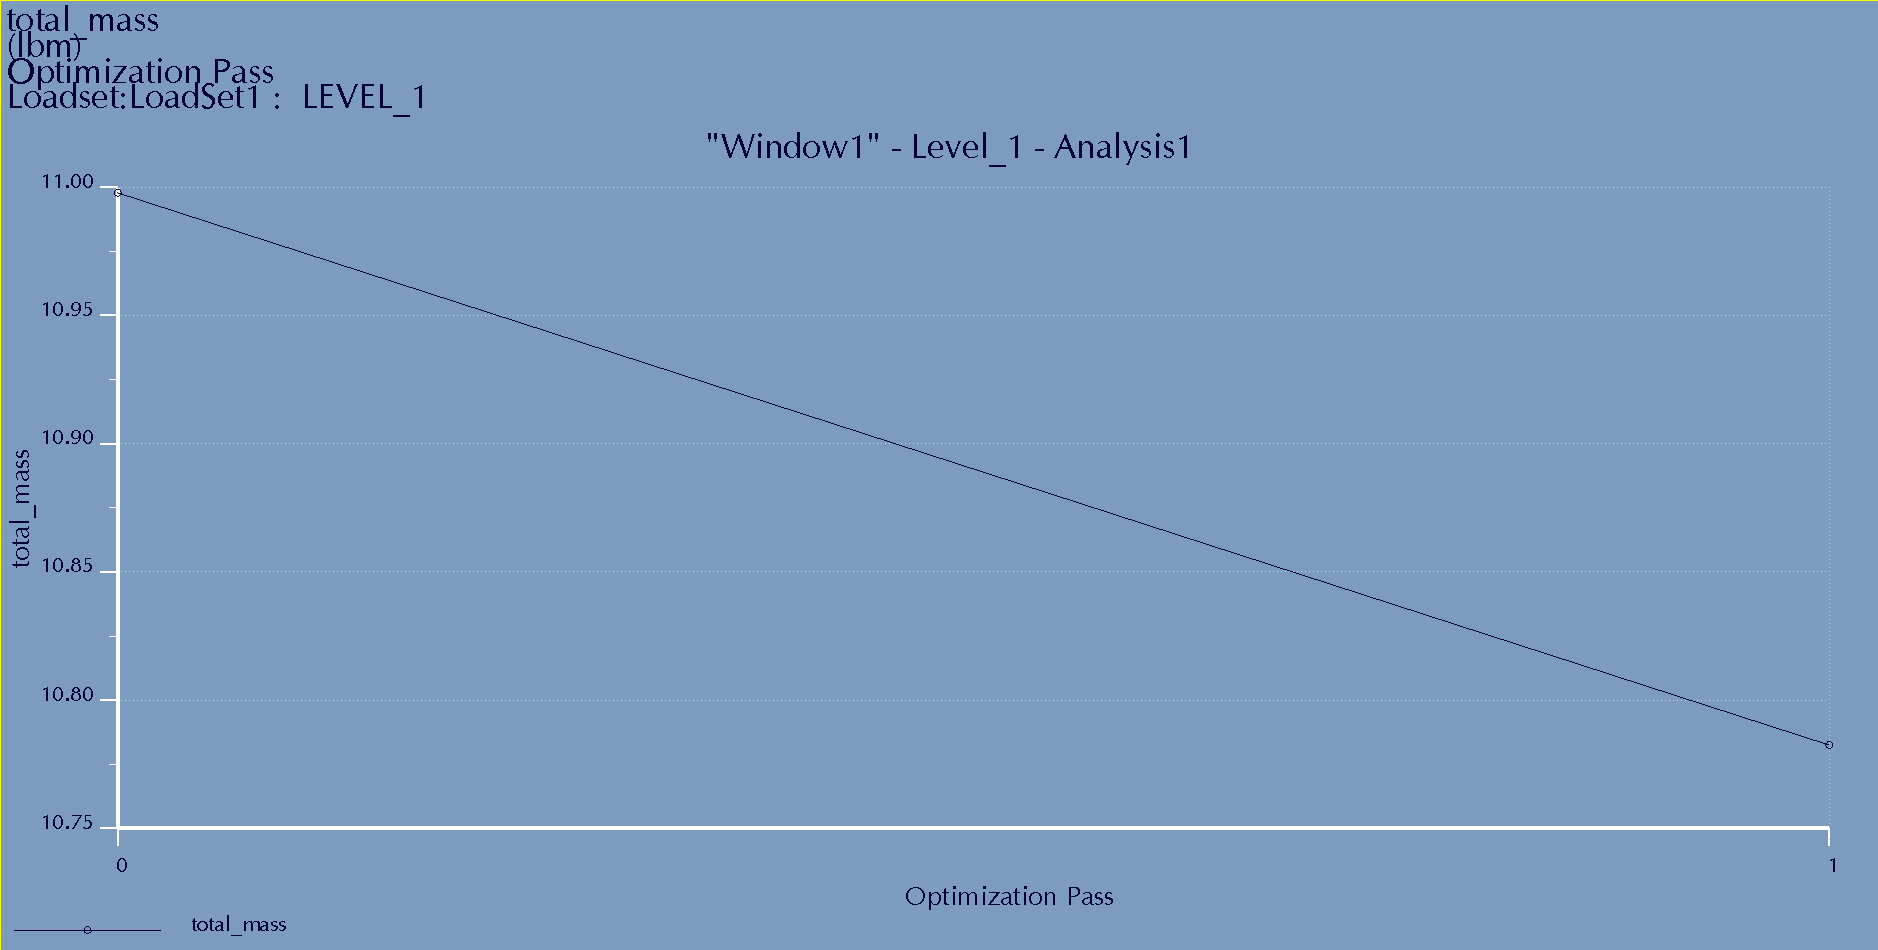
\includegraphics[width=\textwidth]{SinusoidalL1OptimMass}
				\subcaption{Mass}
				\label{fig:L1SinusoidalOptimMassGraph}
			\end{subfigure}
			\caption{Optimization of Level 1 under sinusoidal pressure load}
		\end{figure}
		
		\begin{figure}[H]
			\centering
			\begin{subfigure}{.45\textwidth}
				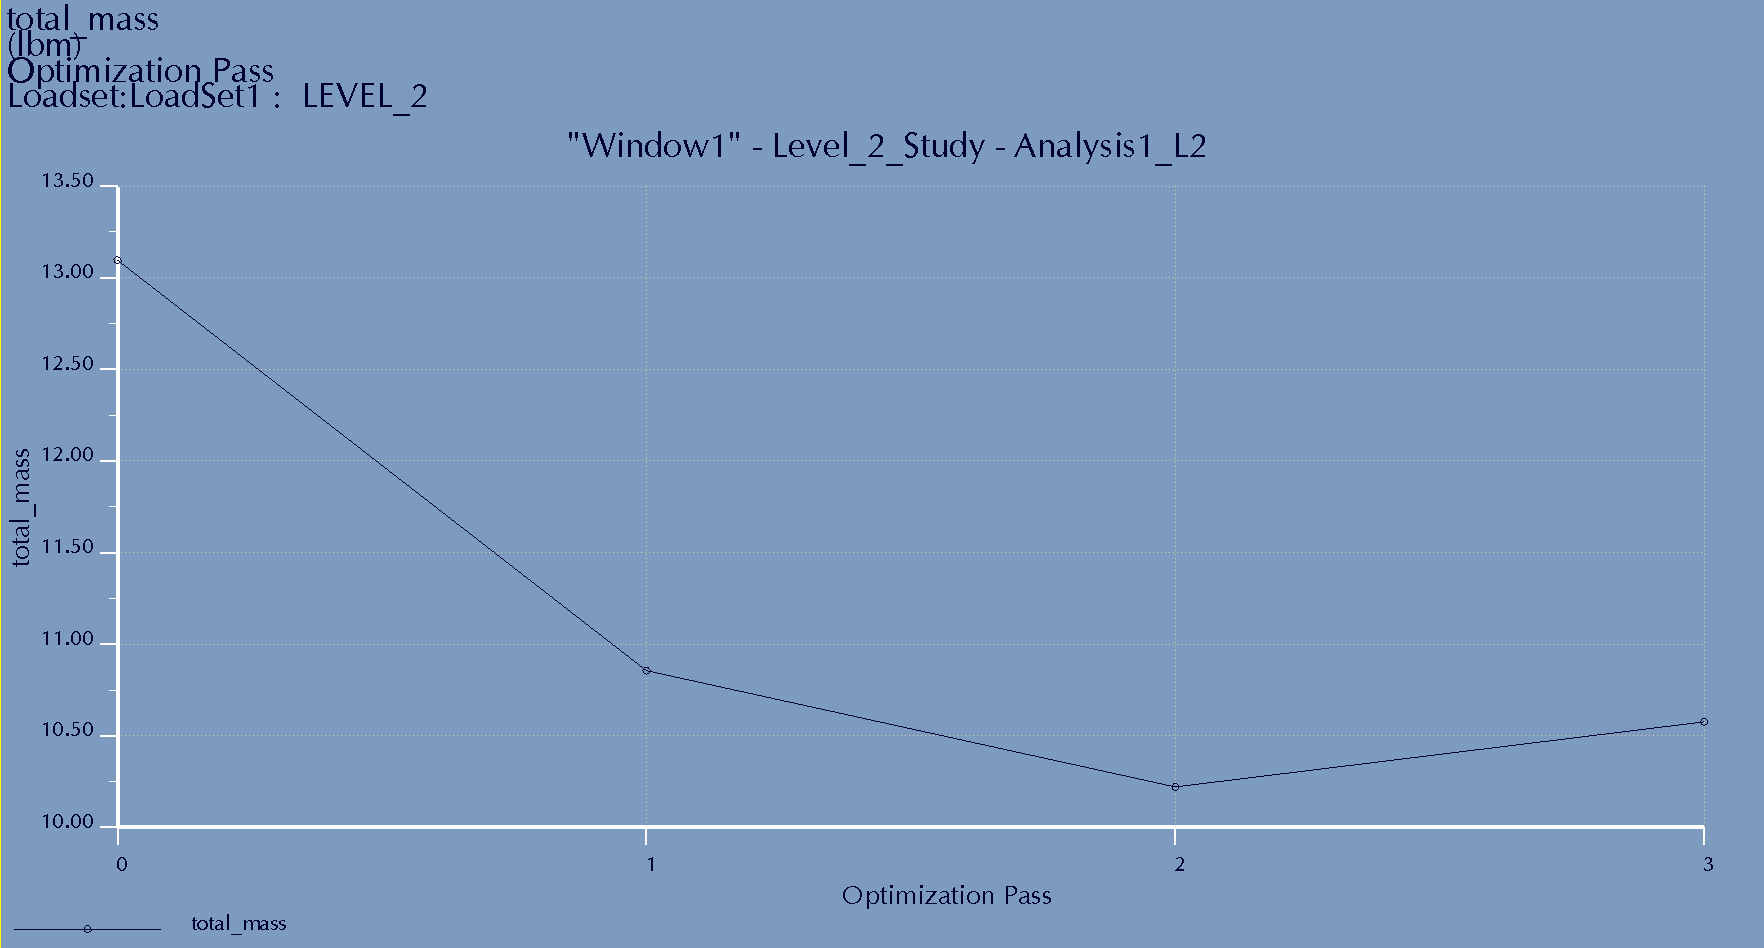
\includegraphics[width=\textwidth]{SinusoidalL2OptimMass}
				\subcaption{Displacement}
				\label{fig:L2SinusoidalOptimDispGraph}
			\end{subfigure}
			\begin{subfigure}{.45\textwidth}
				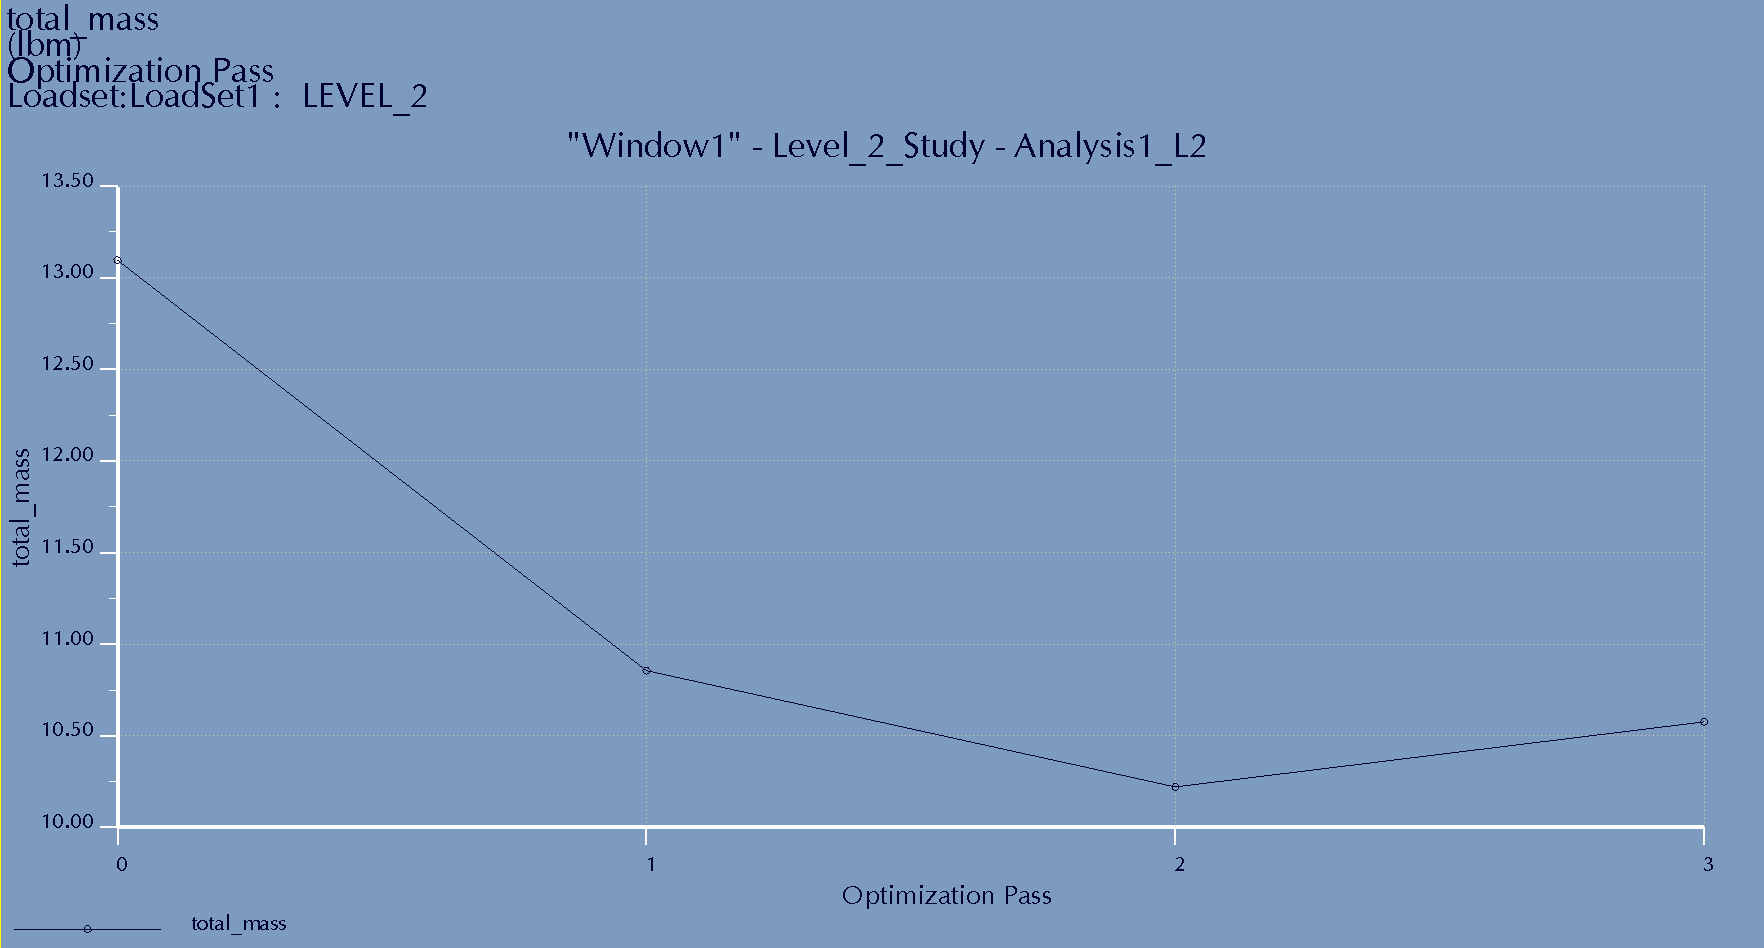
\includegraphics[width=\textwidth]{SinusoidalL2OptimMass}
				\subcaption{Mass}
				\label{fig:L2SinusoidalOptimMassGraph}
			\end{subfigure}
			\caption{Optimization of Level 2 under sinusoidal pressure load}
		\end{figure}
		\graphicspath{ {..} }
		
		
		
		\section{Results of Analysis}
		Table \ref{tab:SummaryOfMass} summarizes the different masses of the louvers after optimization.  Theoretically, for a finished product, a design that meets all of the requirements will be chosen to be purchased and constructed.  In theory, this is the heaviest one, the 1000-psi static force louver.  This design is most likely the strongest and resistant to deformation.  There are, however, possible reasons to choose a different optimization; for instance, 1000 psi on the exterior faces might be considered too strict of a loading requirement.  This would, of course, lead to choosing a different optimization.
		
		\begin{table}[H]
			\centering
			\begin{tabular}{|c|c|}
			\hline \textbf{Force Method} & \textbf{Mass (lbm)}\\
			\hline Bullet & 159.3\\
			\hline 1000 psi Static force & 193.7\\
			\hline 1000 psi Sinusoidal force & 109.8\\
			\hline
			\end{tabular}
			\caption{Summary of masses of three different optimizations}
			\label{tab:SummaryOfMass}
		\end{table}
		
		\begin{center}
			\vfill 
			\begin{scriptsize}
				This space intentionally left blank
			\end{scriptsize}
		\end{center}
		
		\newpage
		\subsection{Bullet Load}
		Figure \ref{fig:BulletDraw} shows the final dimensions of the optimized louver given a continuous force calculated for a 9mm bullet.  Table \ref{tab:BulletDims} tabulates the important measurements of this louver.  Figure \ref{fig:BulletDisp} shows the displacements of a complete louver when impacted with 9mm bullets on each exposed face.  Note that the maximum displacement is $0.50017\inchsign$.
		
		\graphicspath{ {./ScreenShots/Bullet/} }
		\begin{figure}[H]
			\centering
			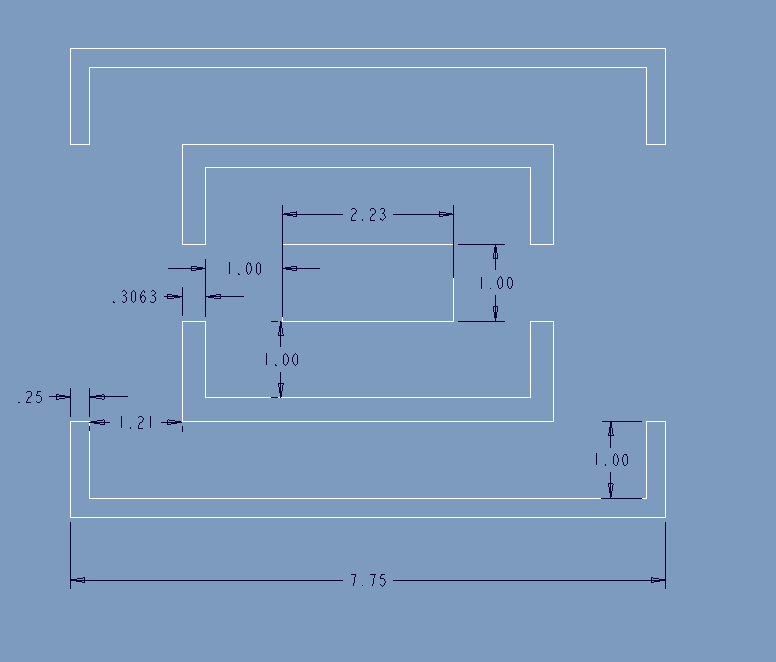
\includegraphics[width=.75\textwidth]{BulletAssyDraw}
			\caption{Drawing showing the dimensions for the bullet load}
			\label{fig:BulletDraw}
		\end{figure}
		
		\begin{figure}[H]
			\centering
			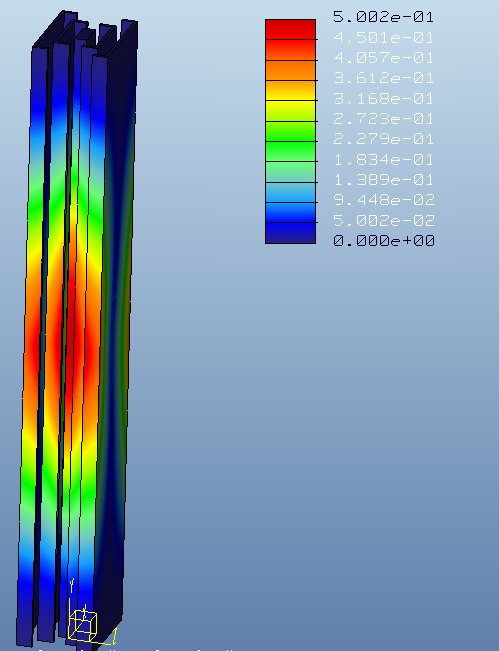
\includegraphics[width=.5\textwidth]{BulletAssyDisp}
			\caption{Displacement under bullet load}
			\label{fig:BulletDisp}
		\end{figure}
		\graphicspath{ {..} }
		
		\begin{table}[H]
			\centering
			\begin{tabular}{|c|c|c|c|}
			\hline \textbf{Dimension} & \textbf{Value (in)} & \textbf{\begin{small}Min Value (in)\end{small}} & \textbf{\begin{small}Max Value (in)\end{small}}\\
			
			\hline Center Thickness & 1.00 & \begin{small}
			1.00
			\end{small} & \begin{small}
			1.00
			\end{small}\\
			
			\hline Center Width & 2.23 & \begin{small}
			0.0625
			\end{small} & \begin{small}
			2.50
			\end{small}\\
			
			\hline
			\hline L1 Thickness & 0.3063 & \begin{small}
			0.125
			\end{small} & \begin{small}
			1.00
			\end{small}\\
			
			\hline L1 Horizontal  & 1.00 & \begin{small}
			1.00
			\end{small} & \begin{small}
			2.00
			\end{small}\\
			
			\hline L1 Vertical  & 1.00 & \begin{small}
			1.00
			\end{small} & \begin{small}
			2.00
			\end{small}\\
			
			\hline
			\hline L2 Thickness & 0.25 & \begin{small}
			0.125
			\end{small} & \begin{small}
			1.00
			\end{small}\\
			
			\hline L2 Horizontal  & 1.21 & \begin{small}
			1.00
			\end{small} & \begin{small}
			2.00
			\end{small}\\
			
			\hline L2 Vertical  & 1.00 & \begin{small}
			1.00
			\end{small} & \begin{small}
			2.00
			\end{small}\\
			
			\hline
			\end{tabular}
			\caption{Summary of dimensions for bullet-optimized louver}
			\label{tab:BulletDims}
		\end{table}
		
		\newpage
		\subsection{Constant Pressure Load}
		Figure \ref{fig:ConstantPressureDraw} shows the final dimensions of the optimized louver given a force over all exposed faces of 1000 psi.  Table \ref{tab:PressureDims} tabulates the important measurements of this louver.  Figure \ref{fig:ConstPressDisp} shows the displacements of a complete louver when loaded with 1000 psi on each exposed face.  Note that the maximum displacement is $0.50832\inchsign$.
		
		\graphicspath{ {./ScreenShots/Pressure/} }
		\begin{figure}[h]
			\centering
			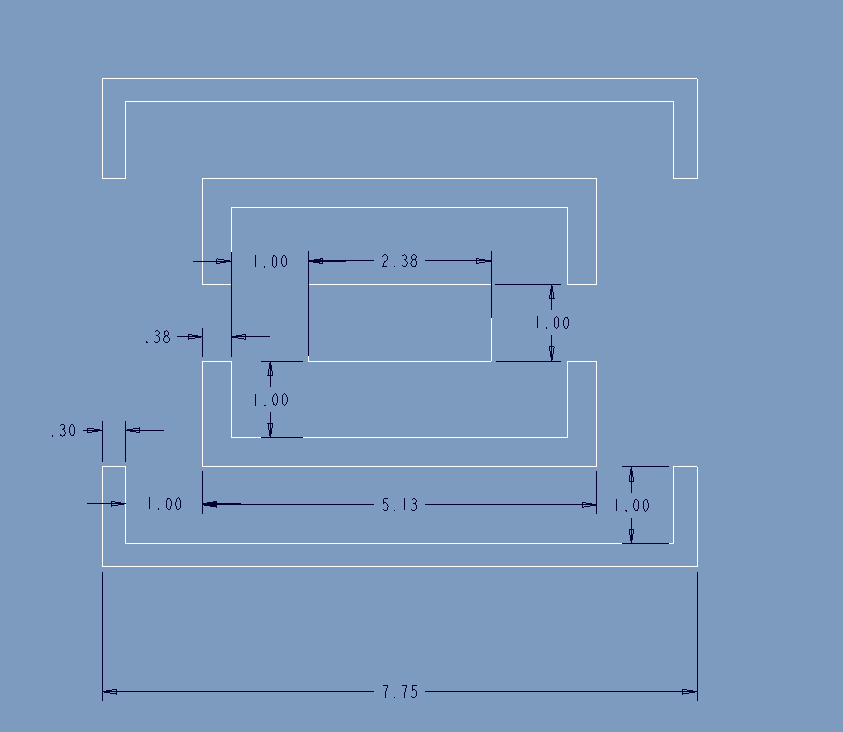
\includegraphics[width=.75\textwidth]{PressureAssyDraw}
			\caption{Drawing showing the dimensions for the constant pressure load}
			\label{fig:ConstantPressureDraw}
		\end{figure}
		
		\begin{figure}[H]
			\centering
			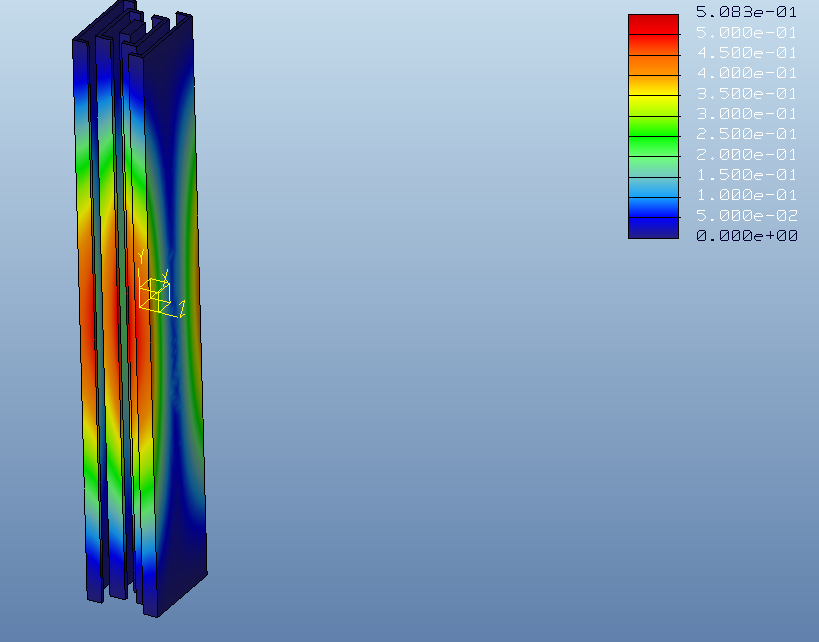
\includegraphics[width=.75\textwidth]{PressAssyDisp}
			\caption{Displacement under constant pressure load}
			\label{fig:ConstPressDisp}
		\end{figure}
		
		\graphicspath{ {..} }
		
		\begin{table}[H]
			\centering
			\begin{tabular}{|c|c|c|c|}
			\hline \textbf{Dimension} & \textbf{Value (in)} & \textbf{\begin{small}Min Value (in)\end{small}} & \textbf{\begin{small}Max Value (in)\end{small}}\\
			
			\hline Center Thickness & 1.00 & \begin{small}
			1.00
			\end{small} & \begin{small}
			1.00
			\end{small}\\
			
			\hline Center Width & 2.38 & \begin{small}
			0.125
			\end{small} & \begin{small}
			3.00
			\end{small}\\
			
			\hline
			\hline L1 Thickness & 0.3063 & \begin{small}
			0.125
			\end{small} & \begin{small}
			1.00
			\end{small}\\
			
			\hline L1 Horizontal  & 1.00 & \begin{small}
			1.00
			\end{small} & \begin{small}
			2.00
			\end{small}\\
			
			\hline L1 Vertical  & 1.00 & \begin{small}
			1.00
			\end{small} & \begin{small}
			2.00
			\end{small}\\
			
			\hline
			\hline L2 Thickness & 0.25 & \begin{small}
			0.125
			\end{small} & \begin{small}
			1.00
			\end{small}\\
			
			\hline L2 Horizontal  & 1.21 & \begin{small}
			1.00
			\end{small} & \begin{small}
			2.00
			\end{small}\\
			
			\hline L2 Vertical  & 1.00 & \begin{small}
			1.00
			\end{small} & \begin{small}
			2.00
			\end{small}\\
			
			\hline
			\end{tabular}
			\caption{Summary of dimensions for louver optimized for constant pressure}
			\label{tab:PressureDims}
		\end{table}
		
		
		\newpage
		\subsection{Sinusoidal Pressure Load}
		Figure \ref{fig:SinusoidPressureDraw} shows the final dimensions of the optimized louver given a force over all exposed faces of 1000 psi.  The blue lines are from the sketches defining the extents of the load.  Figure \ref{fig:SinusoidalPressDisp} shows the displacements of a complete louver when loaded with 1000 psi on each exposed face.  Note that the maximum displacement is $0.5179\inchsign$.  Table \ref{tab:SinusoidDims} tabulates the important measurements of this louver.
		
		\graphicspath{ {./ScreenShots/Sinusoidal/} }
		\begin{figure}[h]
			\centering
			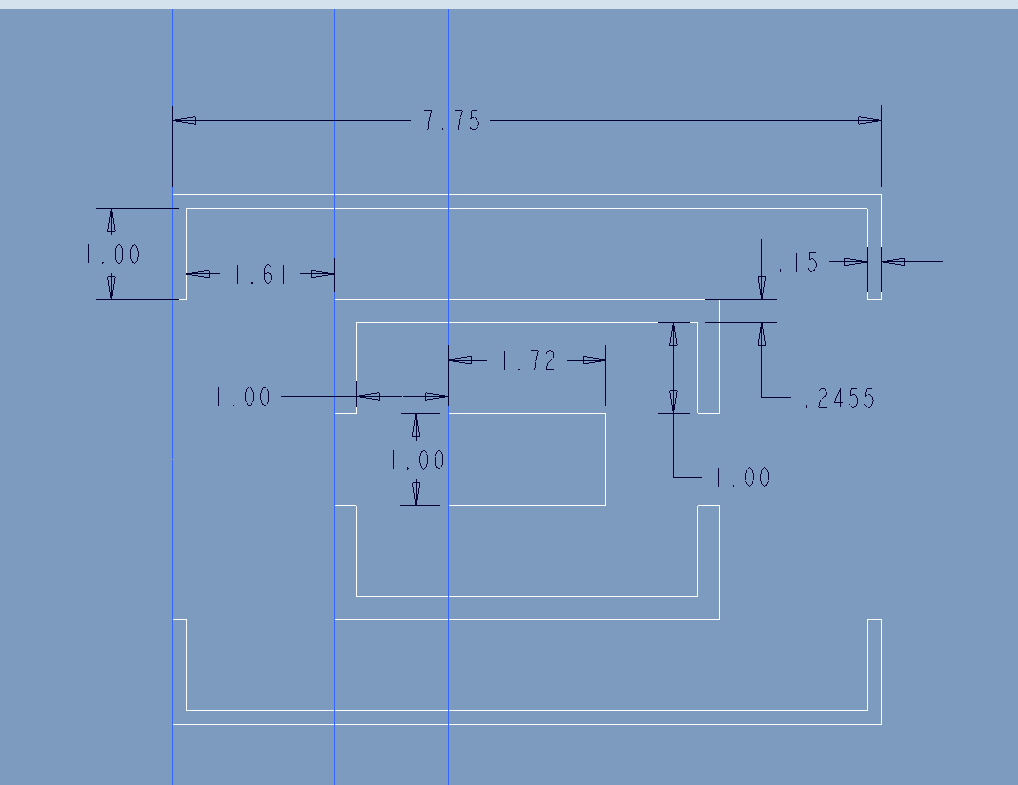
\includegraphics[width=.75\textwidth]{SinusoidalMeasurements}
			\caption{Drawing showing the dimensions for the sinusoidal pressure load}
			\label{fig:SinusoidPressureDraw}
		\end{figure}
		
		\begin{figure}[H]
			\centering
			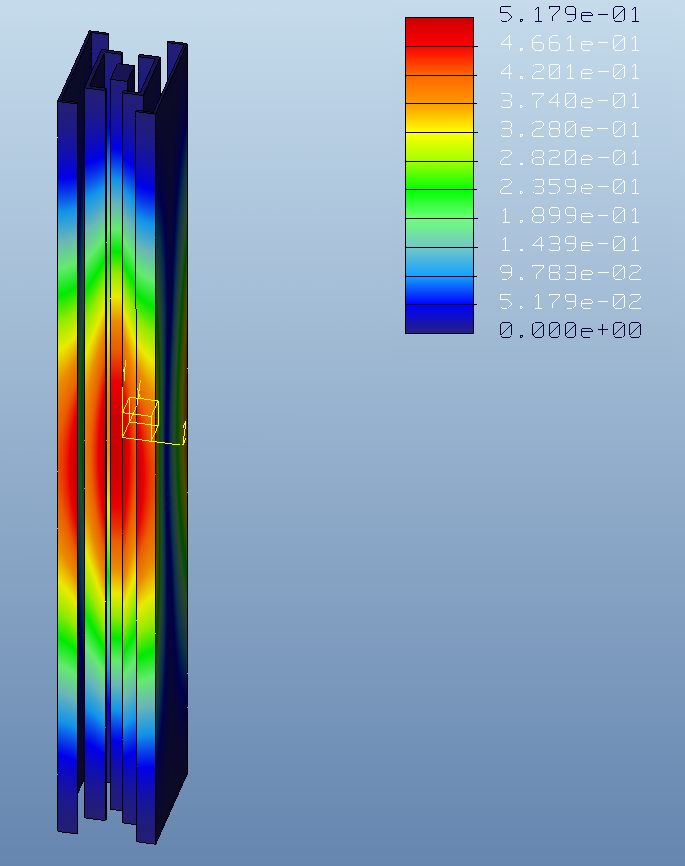
\includegraphics[width=.5\textwidth]{SinusoidalAssyDisp}
			\caption{Displacement under sinusoidal pressure load}
			\label{fig:SinusoidalPressDisp}
		\end{figure}
		\graphicspath{ {..} }
		
		\begin{table}[H]
			\centering
			\begin{tabular}{|c|c|c|c|}
			\hline \textbf{Dimension} & \textbf{Value (in)} & \textbf{\begin{small}Min Value (in)\end{small}} & \textbf{\begin{small}Max Value (in)\end{small}}\\
			
			\hline Center Thickness & 1.00 & \begin{small}
			1.00
			\end{small} & \begin{small}
			1.00
			\end{small}\\
			
			\hline Center Width & 1.72 & \begin{small}
			0.125
			\end{small} & \begin{small}
			2.00
			\end{small}\\
			
			\hline
			\hline L1 Thickness & 0.3063 & \begin{small}
			0.125
			\end{small} & \begin{small}
			1.00
			\end{small}\\
			
			\hline L1 Horizontal  & 1.00 & \begin{small}
			1.00
			\end{small} & 2.00\\
			
			\hline L1 Vertical  & 1.00 & \begin{small}
			1.00
			\end{small} & \begin{small}
			2.00
			\end{small}\\
			
			\hline
			\hline L2 Thickness & 0.25 & \begin{small}
			0.125
			\end{small} & \begin{small}
			1.00
			\end{small}\\
			
			\hline L2 Horizontal  & 1.21 & \begin{small}
			1.00
			\end{small} & \begin{small}
			2.00
			\end{small}\\
			
			\hline L2 Vertical  & 1.00 & \begin{small}
			1.00
			\end{small} & \begin{small}
			2.00
			\end{small}\\
			
			\hline
			\end{tabular}
			\caption{Summary of dimensions for louver optimized for sinusoidal pressure}
			\label{tab:SinusoidDims}
		\end{table}
		
		\chapter{Storm Shutter}
		\vspace{-.25in}
		\section{Overview}
		A storm shutter was designed for use with the FEBR louvers.  The purpose of this shutter is to prevent rain and strong winds from travelling through the louver.  The shutter is not for blast protection.  Figure \ref{fig:ShutterExterior} shows an exterior view of the shutter and Figure \ref{fig:ShutterInterior} shows an interior view of the shutter.
		
		\graphicspath{ {./ScreenShots/Shutter/} }
		\begin{figure}[H]
			\centering
			\begin{subfigure}{.9\textwidth}
				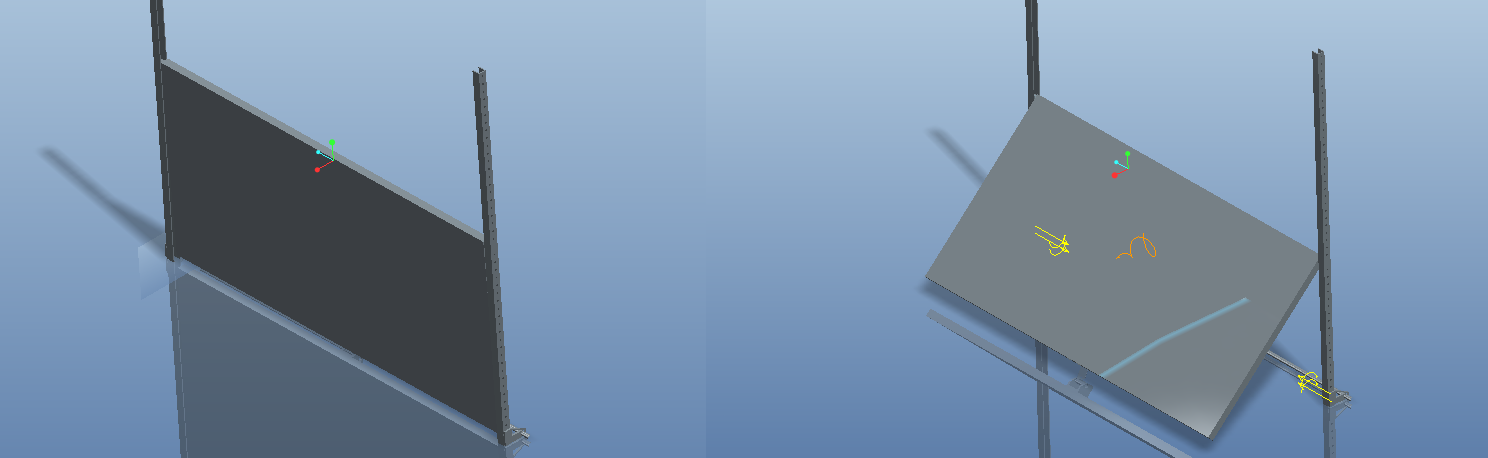
\includegraphics[width=\textwidth]{ShutterExterior}
				\caption{Exterior view of shutter}
				\label{fig:ShutterExterior}
			\end{subfigure}
			\begin{subfigure}{.9\textwidth}
				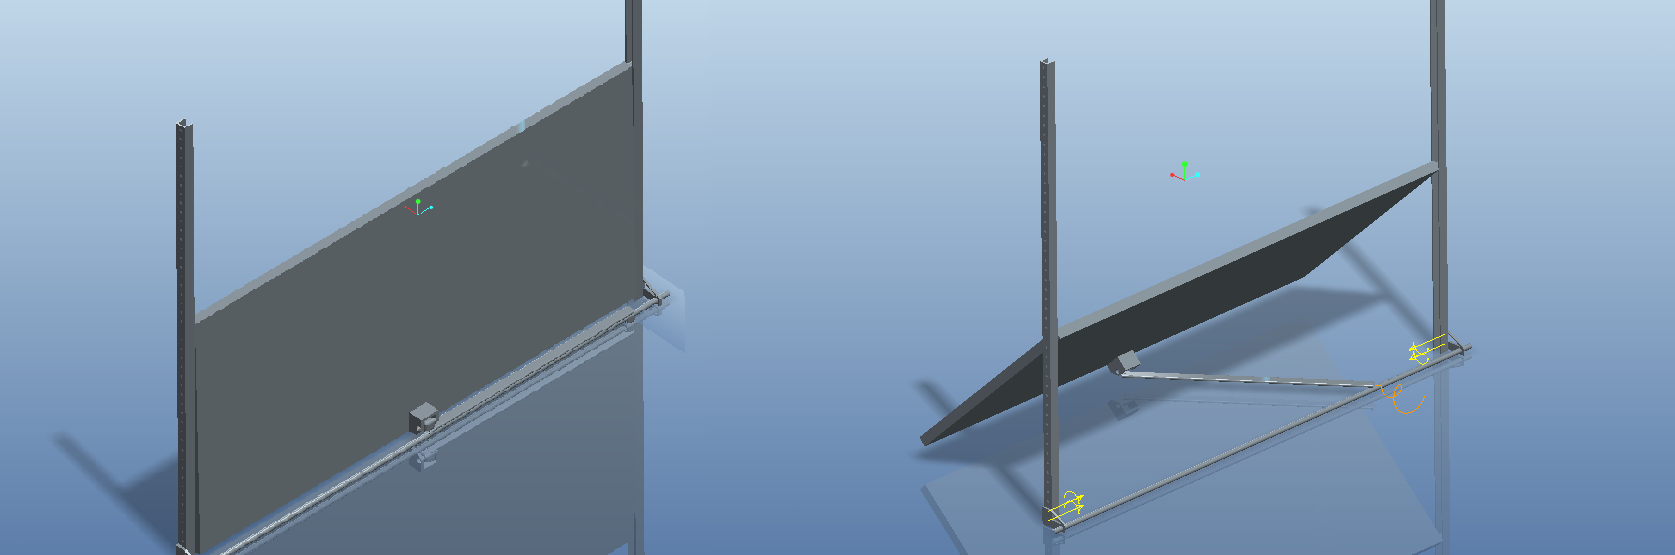
\includegraphics[width=\textwidth]{ShutterInterior}
				\caption{Interior view of shutter}
				\label{fig:ShutterInterior}
			\end{subfigure}
		\end{figure}
		
		Regarding the major dimensions, the shutter is $25\inchsign$ high and $50\inchsign$ wide.  The height allows for two shutters to completely cover one louver completely along its exposed face.  Since the airflow allowed through each individual louver is small because of the one-inch spacing, it is assumed that multiple louvers will be used in a given installation.  The shutter system as designed allows for a high degree of flexibility regarding the height and breadth of the louver system that it must shelter.
		
		Because of the long arm and sliding pivot of the shutter, it requires mechanically few components to cover a large amount of louver while closed; at the same time, it allows a high degree of airflow in clement weather.  Figures \ref{fig:ShutterProfileClose} and \ref{fig:ShutterProfileOpen} show a profile view of the shutter system while closed and opened, respectively.  Note the low degree of air blockage in Figure \ref{fig:ShutterProfileOpen} when opened.
		
		\begin{figure}[H]
			\centering
			\begin{subfigure}{.45\textwidth}
				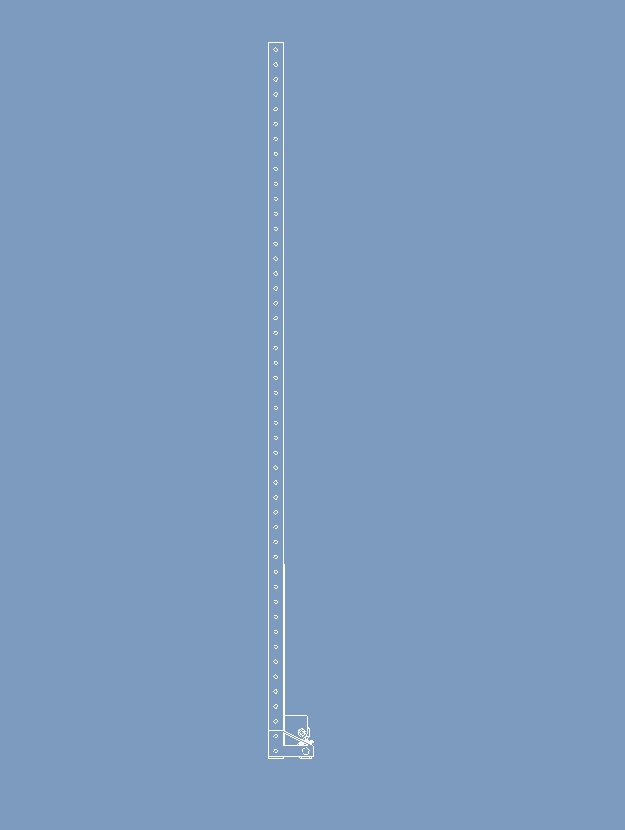
\includegraphics[width=\textwidth]{ShutterAssyDrawClose}
				\caption{Closed}
				\label{fig:ShutterProfileClose}
			\end{subfigure}
			\begin{subfigure}{.45\textwidth}
				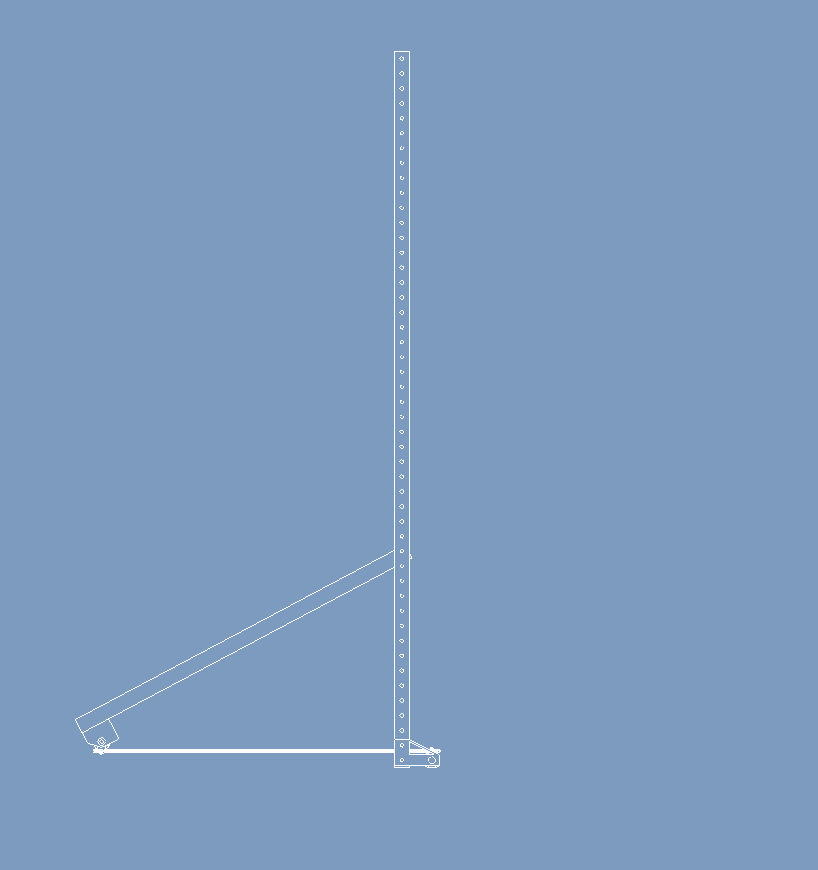
\includegraphics[width=\textwidth]{ShutterAssyDrawOpen}
				\caption{Open}
				\label{fig:ShutterProfileOpen}
			\end{subfigure}
			\caption{Profile view of shutter system}
		\end{figure}
		
		When closed, the shutter is easily smaller than the $6\inchsign$ allotted to it in the specifications.  It is very easy to control the degree to which the shutter opens, discussed in the following section.
		
		\section{Mechanism}
		The chief mechanism by which the shutter is controlled is a threaded rod.  This threaded rod, visible in Figure \ref{fig:ShutterHighlihgtThreadedRod}, controls the horizontal, linear motion of a threaded follower.  This follower then pushes or pulls the shutter into position.  This way, the shutter is held both positively open and closed; it is difficult, if not impossible, to open or close the shutter without either activation or destruction.  While not blast-resistant, a strong, secure shutter system presents a strong, secure fa\c{c}ade for any location installed.
		
		\begin{figure}[h]
			\centering
			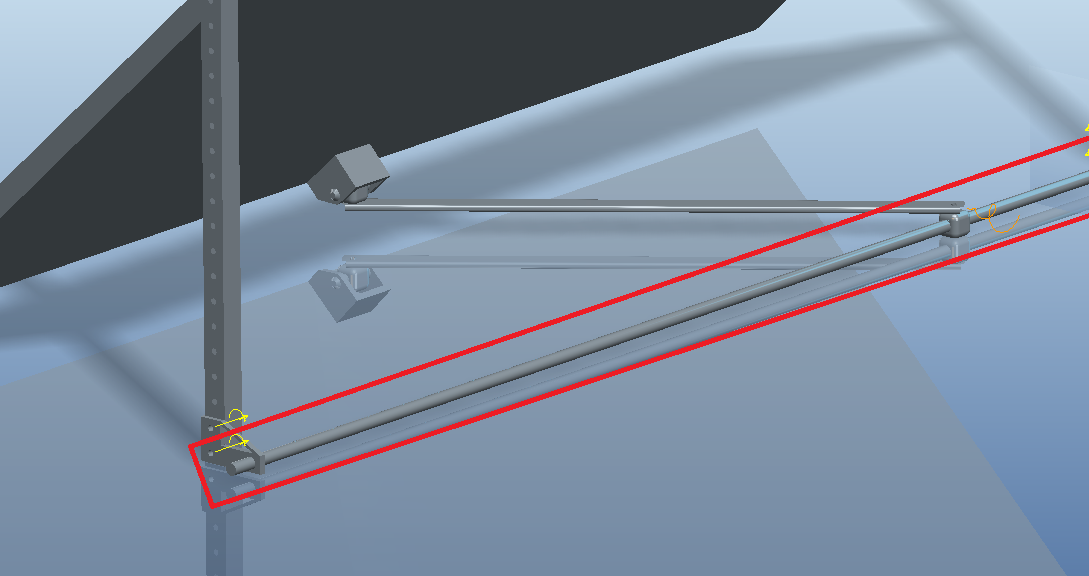
\includegraphics[width=.5\textwidth]{ShutterCloseUpHighlight}
			\caption{Shutter and threaded rod, highlighted in red}
			\label{fig:ShutterHighlihgtThreadedRod}
		\end{figure}
		
		\section{Manufacturing and Installation Flexibility}
		This storm shutter assembly was also designed with manufacturability in mind.  The side supports can simply be extruded aluminum C-channels.  The holes drilled in it are for laser-cut or stamped brackets.  These brackets hold the threaded rod in place and allow for mounting of the control motor.  The location of the bracket determines the lowest point of the shutter, allowing easy installation \textit{in situ}.
		
		Because the rod is easy to use, work with, and source, one motor can control many shutters simultaneously.  Consecutive shutters can be attached to the previous one's threaded rod when they are needed, possibly after construction.  The threaded rods can also accommodate sprockets for chains.  These chains allow for the initial motor to control the shutters above or below the initial one.  This interconnectability and interchangeability among this shutter design allows one motor to control an entire installation of storm shutters.  If redundancy is desired, additional motors can easily be installed, either at the end of an installation at a terminal shutter or at a middle shutter, mounted above the threaded rod running the installation's length.
		
		To minimize friction, Teflon is used between the side C-channels and the sliding sheet.  This Teflon can be added on to the pegs protruding from the sliding sheet, added to the internal surfaces of the channel, or both.
		
		\graphicspath{ {..} }
		\chapter{Conclusions}
		\vspace{-.25in}
		
		An FEBR louver was successfully designed and optimized, given a general starting framework.  A storm shutter to be paired with it was also designed, keeping usability and manufacturability in mind.  Table \ref{tab:SummaryOfMass}, reproduced below, summarizes the masses for the different louvers.  For all of the loading conditions, the maximum deflection was approximately $0.5\inchsign$.  Further analysis, much of it not possible to do with the software provided, is required to determine the optimal configuration of FEBR louver.
		
		\begin{table}[b]
			\centering
			\begin{tabular}{|c|c|}
			\hline \textbf{Force Method} & \textbf{Mass (lbm)}\\
			\hline Bullet & 159.3\\
			\hline 1000 psi Static force & 193.7\\
			\hline 1000 psi Sinusoidal force & 109.8\\
			\hline
			\end{tabular}
			\caption[Summary of masses of three different optimizations]{Summary of masses of three different optimizations (See Table \ref{tab:SummaryOfMass} for context and additional information)}
			\label{tab:SummaryOfMassAgain}
		\end{table}
		
		\newpage
		\newgeometry{margin=1in}
		\chapter{Appendices}
		\section{Appendix A}
		Note that the \texttt{for} loop makes all of the forces outside of the 10-inch radius circle equal to zero.  Although the function is defined for all real numbers, only the forces in the 20-inch diameter circle are of concern.
			\matlabscript{ForcePlot}{}
\end{document}